% =====================================================================
%  legoESM -- Supplementary Information
%  Compile: pdflatex -> bibtex -> pdflatex -> pdflatex
% =====================================================================
\documentclass[11pt]{article}

\usepackage[utf8]{inputenc}
\usepackage[T1]{fontenc}
\usepackage{lmodern}
\usepackage[margin=1in]{geometry}
\usepackage{amsmath,amssymb,bm,mathtools}
\usepackage{graphicx}
\usepackage{subcaption}
\usepackage{booktabs}
\usepackage{longtable}
\usepackage{array}
\usepackage{xcolor}
\usepackage{listings}
\usepackage[numbers,super,sort&compress]{natbib}
\usepackage[colorlinks=true,allcolors=blue!55!black]{hyperref}

\graphicspath{{figures/}}

% number SI figures/tables/equations with an "S" prefix
\renewcommand{\thefigure}{S\arabic{figure}}
\renewcommand{\thetable}{S\arabic{table}}
\renewcommand{\theequation}{S\arabic{equation}}
\renewcommand{\thesection}{S\arabic{section}}

% math shortcuts
\newcommand{\dd}{\mathrm{d}}
\newcommand{\pp}{\partial}
\newcommand{\half}{\tfrac{1}{2}}
\newcommand{\Rd}{R_d}
\newcommand{\Lv}{L_v}
\newcommand{\vect}[1]{\bm{#1}}
\newcommand{\grad}{\nabla}
\newcommand{\divg}{\nabla\!\cdot\!}
\newcommand{\curl}{\nabla\!\times\!}

\lstset{basicstyle=\ttfamily\footnotesize,breaklines=true,frame=single,
        framerule=0.3pt,backgroundcolor=\color{black!3},columns=fullflexible,
        keepspaces=true,language=Python,showstringspaces=false}

\title{\textbf{Supplementary Information for\\[2pt]
legoESM: a composable, differentiable, multi-scale Earth system model built with AI agents}}
\author{}
\date{}

\begin{document}
\maketitle
\vspace{-2.2em}
\tableofcontents
\bigskip
\hrule
\bigskip

\noindent This Supplement provides (\S1) a self-contained description of the governing
equations and numerical methods; (\S2) dynamical-core verification; (\S3) composability
details; (\S4) the large-eddy and cloud-resolving suites; (\S5) ocean validation; (\S6)
performance and scaling; (\S7) accessibility and a code example; and (\S8) operator-level
physical-consistency tests. A complete treatment is in the legoESM Scientific Guide that ships
with the source code\cite{Kochkov2024}.

% #####################################################################
\section{Model description: governing equations and numerics}
% #####################################################################
legoESM is a federation of packages sharing one namespace under a one-way dependency graph
(\texttt{core} $\prec$ \{\texttt{atmosphere}, \texttt{ocean}, \texttt{land}, \texttt{ice}\}
$\prec$ \{\texttt{coupler}, \texttt{ml}, \texttt{tools}\}; main-text Fig.~1). All code is
pure-functional JAX; time integration uses \texttt{lax.scan}; spectral cores use
\texttt{float64}/\texttt{complex128} while finite-volume cores may use \texttt{float32}.

% ----------------------------------------------------------
\subsection{Grids and vertical coordinates}
\paragraph{Cubed sphere.} Six faces are mapped to the sphere by an equiangular gnomonic
projection\cite{Ronchi1996,PutmanLin2007}. With equiangular coordinates
$(\alpha_x,\alpha_y)\in[-\pi/4,\pi/4]^2$ the cell area on a C$n$ face is
\begin{equation}
\Delta A=\frac{R^2\,\Delta\alpha^2}{\cos^2\!\alpha_x\,\cos^2\!\alpha_y\,D^3},\qquad
D=\sqrt{1+\tan^2\!\alpha_x+\tan^2\!\alpha_y},\qquad \Delta\alpha=\frac{\pi}{2n},
\end{equation}
and integrating over the six faces recovers $4\pi R^2$ to round-off (discrete area
conservation). Vector halo exchange rotates to geographic components across panel seams; a
duo-grid treatment of the edges removes the residual differential-operator imprint\cite{Mouallem2023}.

\paragraph{Spectral/Gaussian.} Fields are represented by spherical-harmonic coefficients with
triangular truncation at total wavenumber $n_{\max}$\cite{Bourke1972}. Analysis is an FFT in
longitude followed by Gaussian quadrature in latitude with the fully normalized associated
Legendre functions $P_n^m$. The Laplacian is diagonal, $\nabla^2\hat f_{nm}=-n(n+1)/a^2\,\hat
f_{nm}$, giving exact, grid-imprint-free linear operators and hyperdiffusion
$-\nu[n(n+1)/a^2]^p$.

\paragraph{Voronoi/MPAS.} An unstructured centroidal Voronoi tessellation with mimetic TRiSK
operators\cite{Thuburn2009,Ringler2010,Skamarock2012}: scalars at cell centres, normal velocity
at edges, vorticity at vertices, with
\begin{equation}
(\divg\vect{u})_c=\frac{1}{A_c}\sum_e n_{e,c}u_e l_e,\quad
(\grad\phi)_e=\frac{\phi_{c_2}-\phi_{c_1}}{d_e},\quad
(\curl\vect{u})_v=\frac{1}{A_v}\sum_e t_{e,v}u_e d_e .
\end{equation}

\paragraph{Vertical coordinates.} The atmosphere uses sigma $\sigma=p/p_s$ or hybrid
sigma--pressure $p(k)=A(k)p_{\mathrm{ref}}+B(k)p_s$; geopotential uses the energy-conserving
Simmons--Burridge discretization\cite{SimmonsBurridge1981}
\begin{equation}
\Phi_k=\Phi_s+\Rd\!\!\sum_{k'=k+1}^{N-1}\!T_{k'}\ln\frac{\sigma_{k'+1/2}}{\sigma_{k'-1/2}}
+\alpha_k\Rd T_k,\qquad
\alpha_k=1-\frac{\sigma_{k-1/2}}{\Delta\sigma_k}\ln\frac{\sigma_{k+1/2}}{\sigma_{k-1/2}} .
\end{equation}
The ocean uses a dynamic $z^\ast$ coordinate with free surface $\eta$ and layer Jacobian
$J(\eta)=(\eta+H)/H_{\max}$.

% ----------------------------------------------------------
\subsection{Atmospheric dynamics}
\paragraph{Shallow water (vector-invariant).}
\begin{equation}
\frac{\pp h}{\pp t}=-\divg(h\vect{v}),\quad
\frac{\pp u}{\pp t}=(\zeta+f)v-\frac{\pp B}{\pp x}+D_u,\quad
\frac{\pp v}{\pp t}=-(\zeta+f)u-\frac{\pp B}{\pp y}+D_v,
\end{equation}
with Bernoulli function $B=\half(u^2+v^2)+g(h+h_s)$ and relative vorticity $\zeta$. On the
cubed sphere the FV3-style C-D grid carries momentum on the D-grid and diagnoses C-grid mass
fluxes, with PPM transport\cite{ColellaWoodward1984,Lin2004,PutmanLin2007}; the
circulation-based corner vorticity removes the Hollingsworth--K\"allberg instability.

\paragraph{Hydrostatic primitive equations ($\sigma$).}
\begin{align}
\frac{\pp p_s}{\pp t}&=-\!\int_0^1\!\divg(p_s\vect{v})\,\dd\sigma,\\
\frac{\pp u}{\pp t}&=(\zeta+f)v-\frac{\pp B}{\pp x}-\Rd T\frac{\pp\ln p_s}{\pp x}+D_u,\\
\frac{\pp T}{\pp t}&=-\divg(T\vect{v})+T\divg\vect{v}-\dot\sigma\frac{\pp T}{\pp\sigma}
+\kappa T\frac{\omega}{p}+Q,
\end{align}
with $\kappa=\Rd/c_p$ and diabatic heating $Q$ from physics. The spectral core advances the
vorticity--divergence form with the fast gravity-wave terms treated semi-implicitly
\cite{HoskinsSimmons1975}, yielding a per-wavenumber Helmholtz solve pre-factored at
initialization. The nonhydrostatic core integrates the fully compressible Euler equations on a
terrain-following height coordinate for CRM/LES use.

\paragraph{Coupling.} legoESM uses time-split coupling: the dynamical core updates the state,
then the physics pipeline applies parameterizations in the order radiation $\rightarrow$ deep
convection $\rightarrow$ shallow convection/large-scale condensation $\rightarrow$ microphysics
$\rightarrow$ boundary-layer turbulence $\rightarrow$ gravity-wave drag $\rightarrow$ surface
fluxes, followed by conservation fixers and diagnostics. A grid-agnostic column adapter reshapes
any grid's 3D state to $(n_\mathrm{col},n_\mathrm{lev})$ for physics.

% ----------------------------------------------------------
\subsection{Atmospheric physics (selected closures)}
Radiation is either gray (Frierson-style\cite{Frierson2006}) or correlated-$k$
RRTMGP\cite{Pincus2019}. Mass-flux convection (Tiedtke\cite{Tiedtke1989},
Zhang--McFarlane\cite{ZhangMcFarlane1995}, Bechtold, Kain--Fritsch, Emanuel, Kuo, EDMF, SBM)
shares a unified updraft core. Surface exchange uses Monin--Obukhov similarity; boundary-layer
mixing offers Louis, Holtslag--Boville, YSU, EDMF, TKE and Smagorinsky\cite{Smagorinsky1963}
options. Warm-rain microphysics ranges from Kessler to two-moment schemes and a super-droplet
method\cite{Shima2009}. Each scheme is a factory returning
$\texttt{physics\_fn}(\text{state},\text{grid},\text{coord})\!\to\!\text{tendencies}$, and the
combined tendency is the exact sum of the enabled processes.

% ----------------------------------------------------------
\subsection{Ocean}
The ocean solves the hydrostatic Boussinesq primitive equations with a split-explicit
free-surface barotropic solver\cite{ShchepetkinMcWilliams2005}, KPP vertical
mixing\cite{LMD1994}, GM--Redi isopycnal/eddy mixing\cite{GM1990}, and a TEOS-10-style
polynomial equation of state. Tracers obey
$\pp_t(h\theta)+\divg(h\vect{u}\theta)=\divg(h\,\mathbf{K}\grad\theta)+\mathcal{S}_\theta$,
with $h$ the layer thickness and $\mathbf{K}$ the (rotated) diffusivity tensor. The barotropic
subsystem is advanced either implicitly (Crank--Nicolson) or by a SOTA split-explicit substep
with local CFL clamping; both conserve volume and tracers to the gated tolerance.

% ----------------------------------------------------------
\subsection{Land, sea ice, coupler, ML}
The multi-layer land model solves the mixed-form Richards
equation\cite{VanGenuchten1980} for soil moisture, Johansen thermal diffusion for soil
temperature, Farquhar--Ball-Berry photosynthesis\cite{Farquhar1980} with stomatal conductance,
and a DALEC-style carbon cycle. Sea ice uses EVP/mEVP
rheology\cite{HunkeDukowicz1997} with a multi-category thickness distribution and
energy-conserving thermodynamics. The coupler exchanges area-weighted surface fluxes over
sub-grid tiles with a Monin--Obukhov surface layer. The \texttt{ml} package provides spherical
Fourier neural operators\cite{Bonev2023} (built on Fourier neural operators\cite{Li2021}),
conservation-aware losses, differentiable training drivers, and variational (4D-Var) data
assimilation that differentiates through the compiled time-stepping kernel.

% #####################################################################
\section{Dynamical-core verification}
% #####################################################################
legoESM is gated on the standard sphere test
set\cite{Williamson1992,JablonowskiWilliamson2006,HeldSuarez1994}. Figure~\ref{si:cosinebell}
shows cosine-bell solid-body advection (Williamson case 1) on the cubed sphere; the bell
traverses panel edges without distortion. Figure~\ref{si:w5w6} shows the Williamson 5
(flow over an isolated mountain) and Williamson 6 (Rossby--Haurwitz wave) tests on the
cubed sphere. The Jablonowski--Williamson baroclinic wave is shown for surface pressure and
near-surface wind speed in Fig.~\ref{si:baroclinic}. Crucially, because the equation set and the
numerical discretization are independent choices in legoESM, the same shallow-water problem can
be solved on every grid: Fig.~\ref{si:gridcompare} shows that the cubed-sphere, lat--lon,
icosahedral and spectral cores give visually indistinguishable solutions for the
Rossby--Haurwitz wave and for flow over a mountain. Mass is conserved to round-off; energy and
potential enstrophy budgets close to their scheme-dependent tolerances.

\begin{figure}[h]\centering
\begin{subfigure}{0.495\textwidth}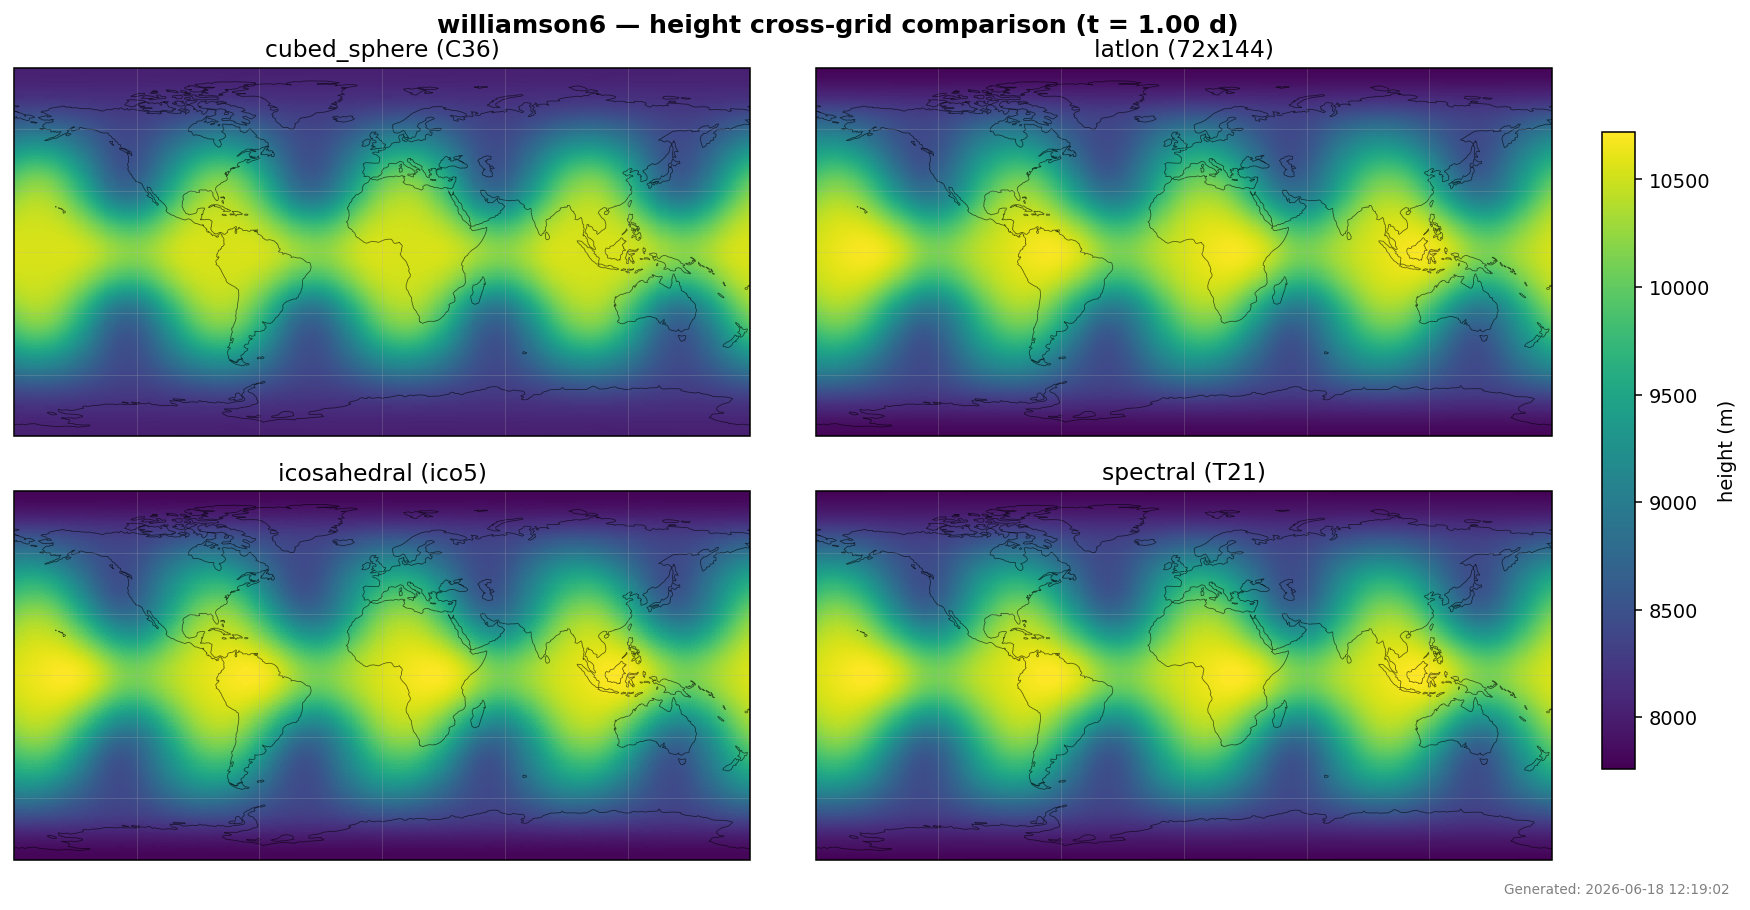
\includegraphics[width=\textwidth]{si_grids_w6.png}
\caption{Williamson 6 (Rossby--Haurwitz wave)}\end{subfigure}\hfill
\begin{subfigure}{0.495\textwidth}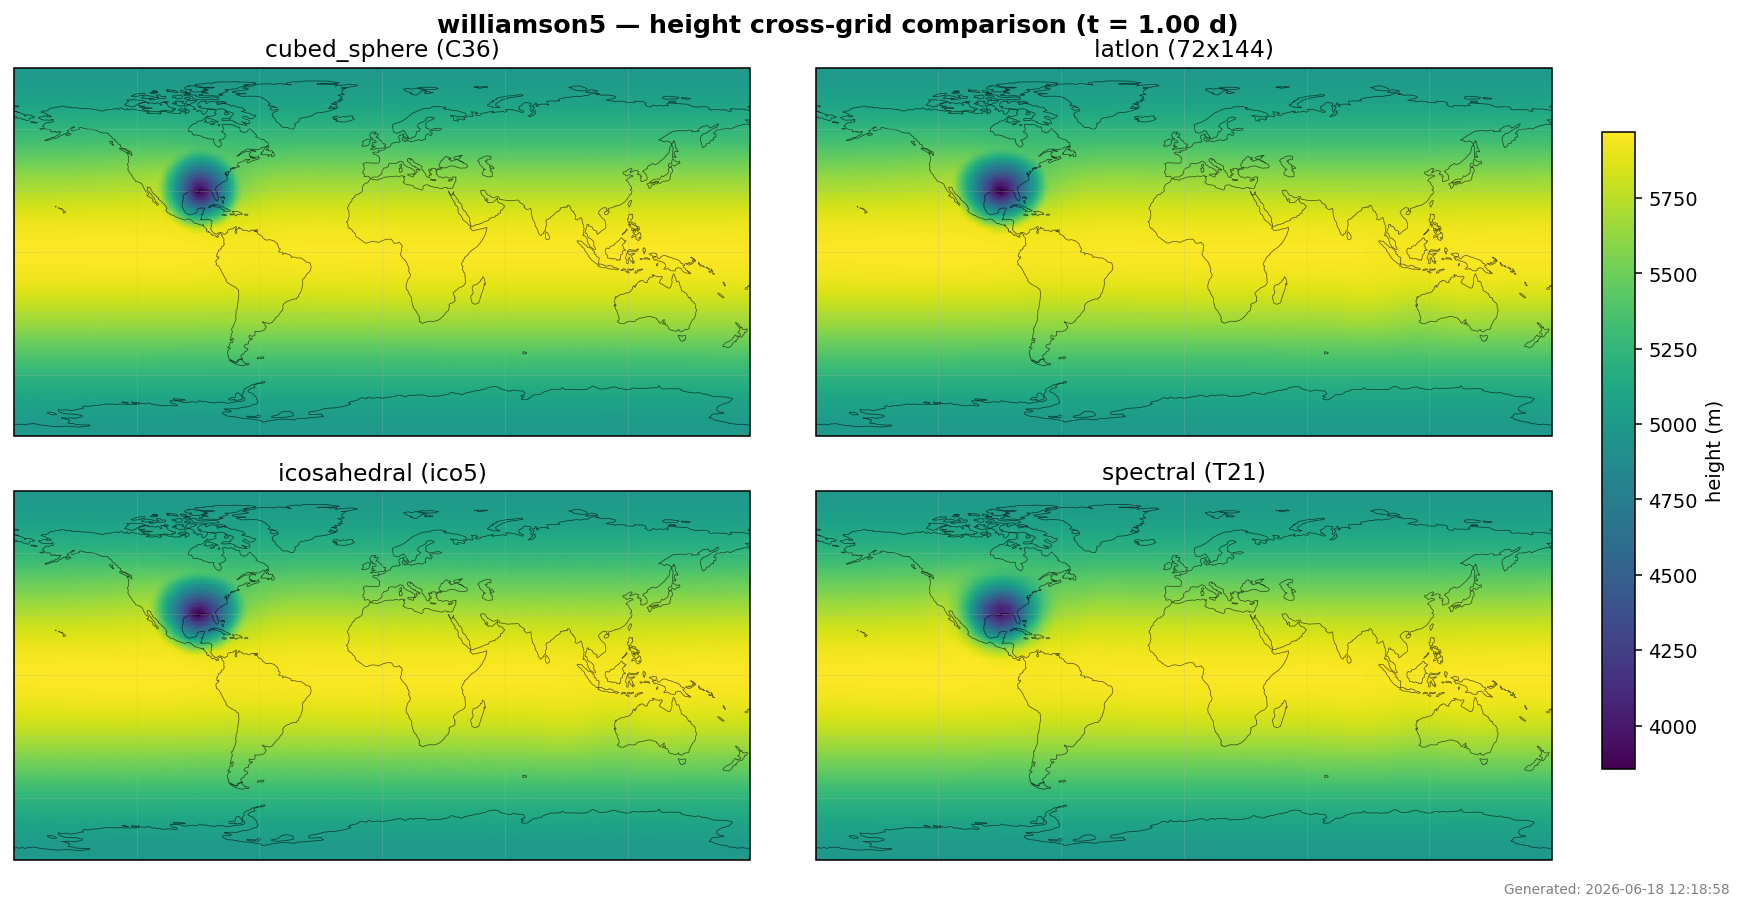
\includegraphics[width=\textwidth]{si_grids_w5.png}
\caption{Williamson 5 (flow over a mountain)}\end{subfigure}
\caption{\textbf{The same shallow-water equations solved on four grids.} Height field for (a) the
Rossby--Haurwitz wave (Williamson 6) and (b) flow over an isolated mountain (Williamson 5), each
integrated on the cubed-sphere (C36), lat--lon ($72\times144$), icosahedral (level~5) and
spectral (T21) discretizations. The solutions are visually indistinguishable across grids,
showing that the physical equation set and the numerical method are orthogonal choices
\cite{Williamson1992}.}\label{si:gridcompare}
\end{figure}

\begin{figure}[h]\centering
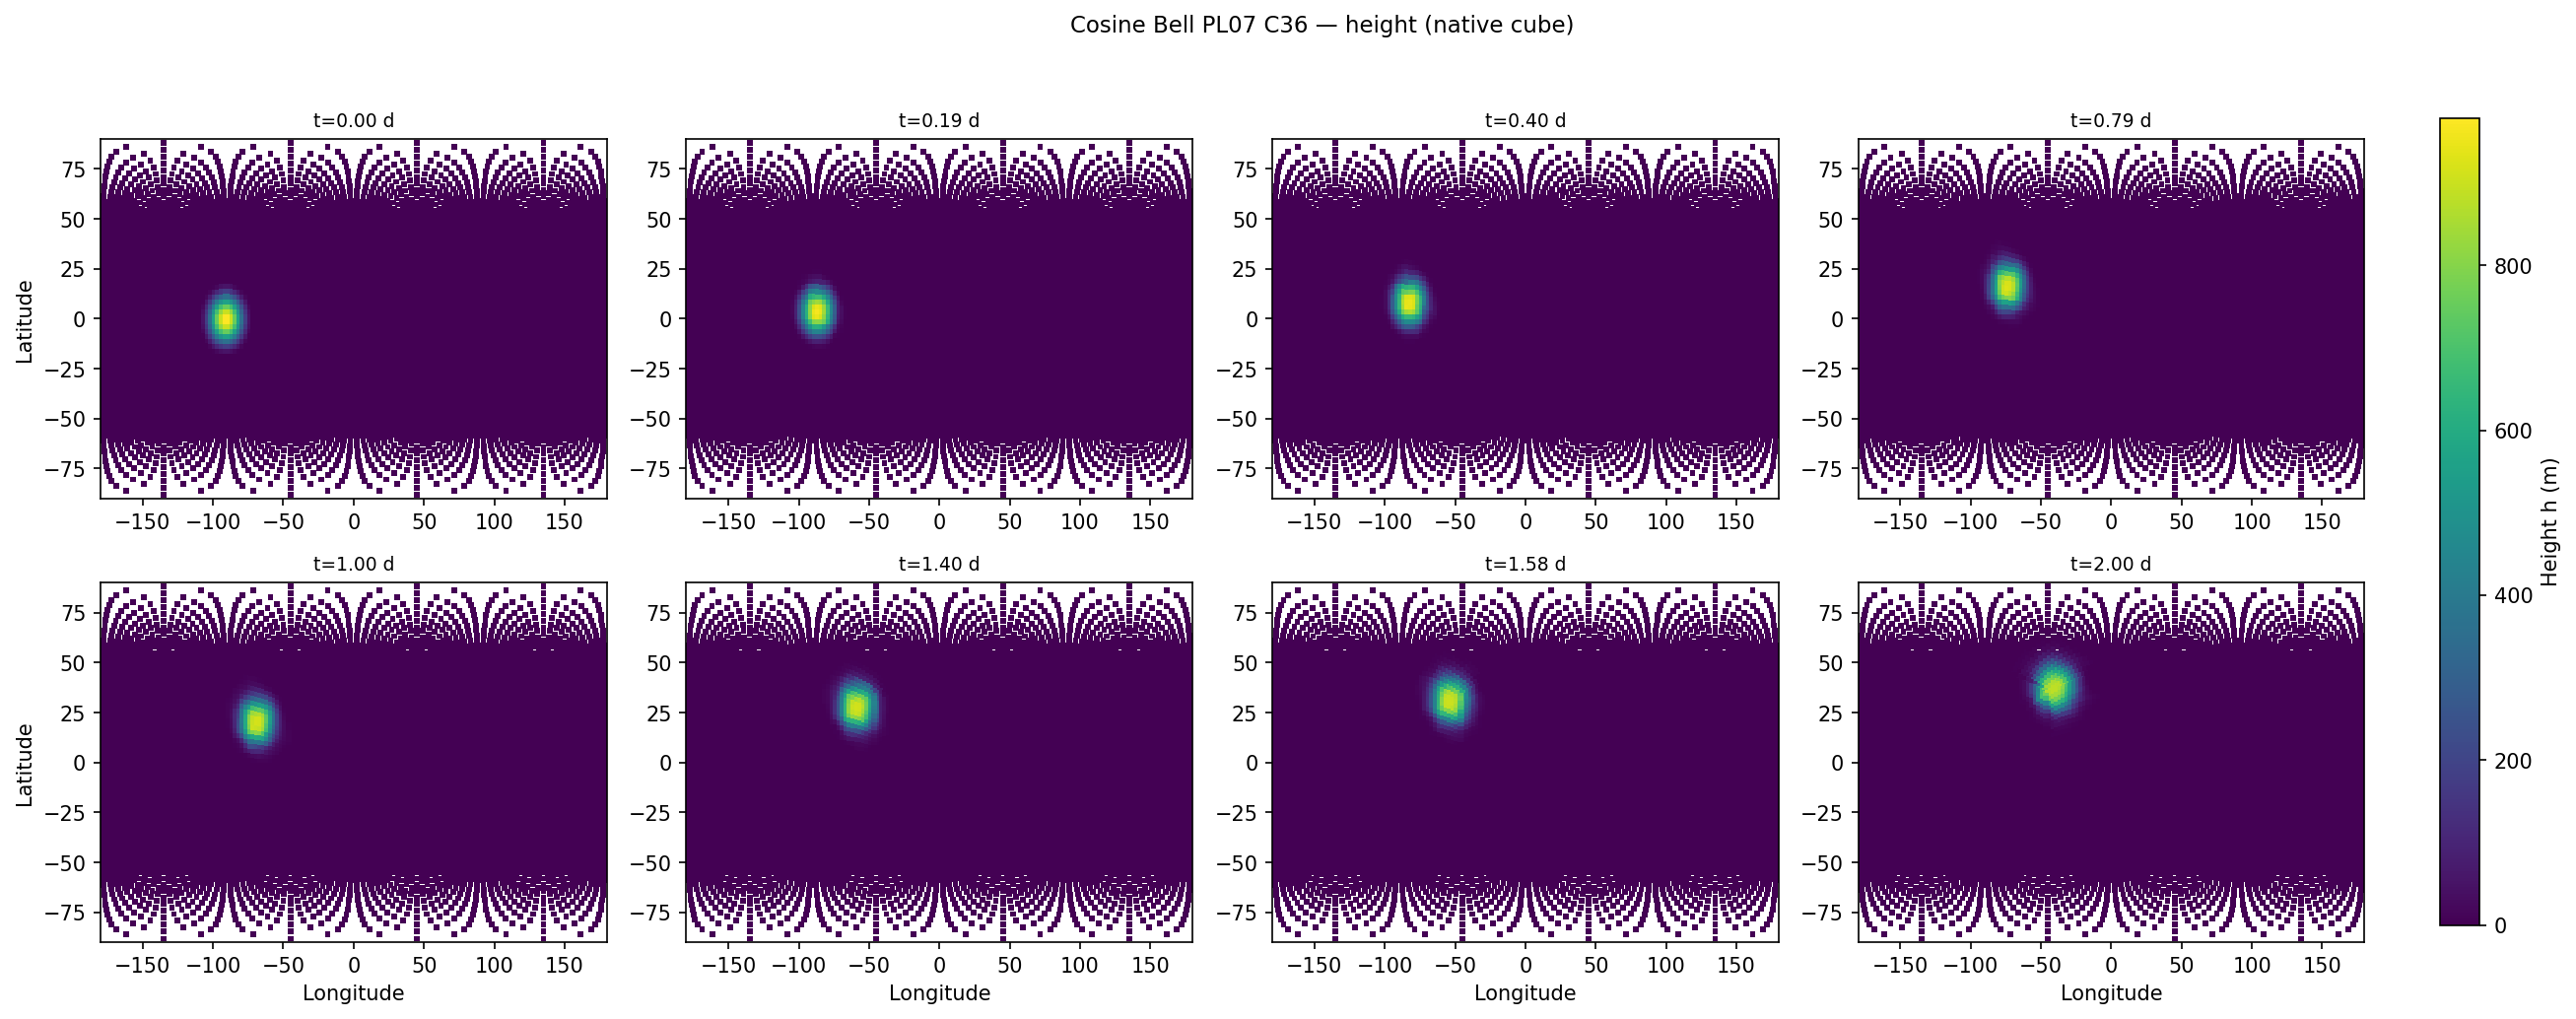
\includegraphics[width=0.92\textwidth]{si_cosinebell.png}
\caption{Cosine-bell advection (Williamson case 1) on the cubed sphere (C36), shown in the
lat--lon projection at successive times. The tracer maintains its shape and amplitude as it
crosses cube-panel edges.}\label{si:cosinebell}
\end{figure}

\begin{figure}[h]\centering
\begin{subfigure}{0.495\textwidth}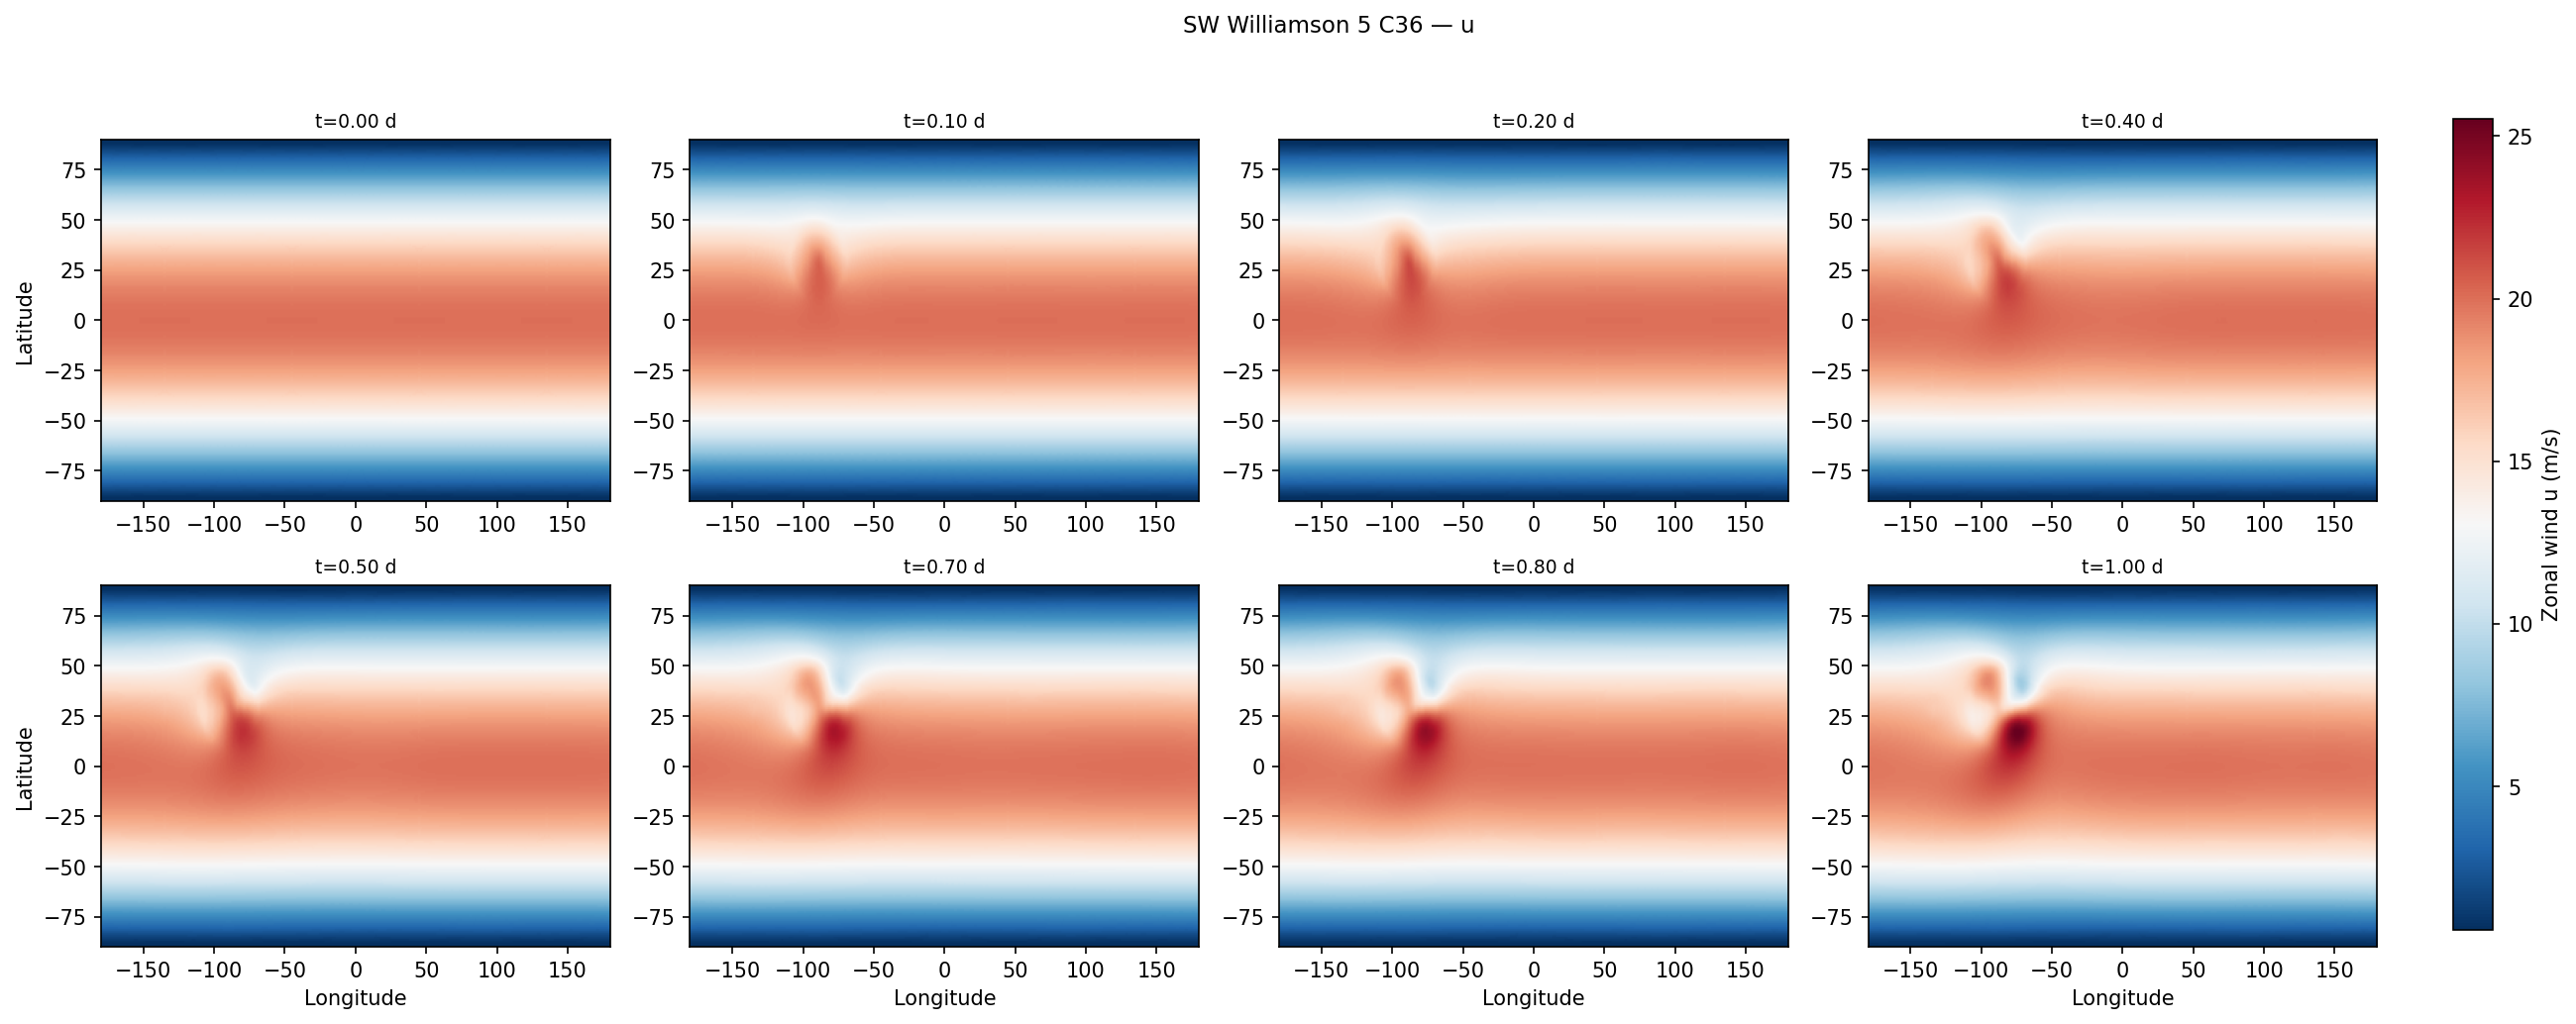
\includegraphics[width=\textwidth]{si_sw_w5_cube.png}
\caption{Williamson 5 (flow over a mountain)}\end{subfigure}\hfill
\begin{subfigure}{0.495\textwidth}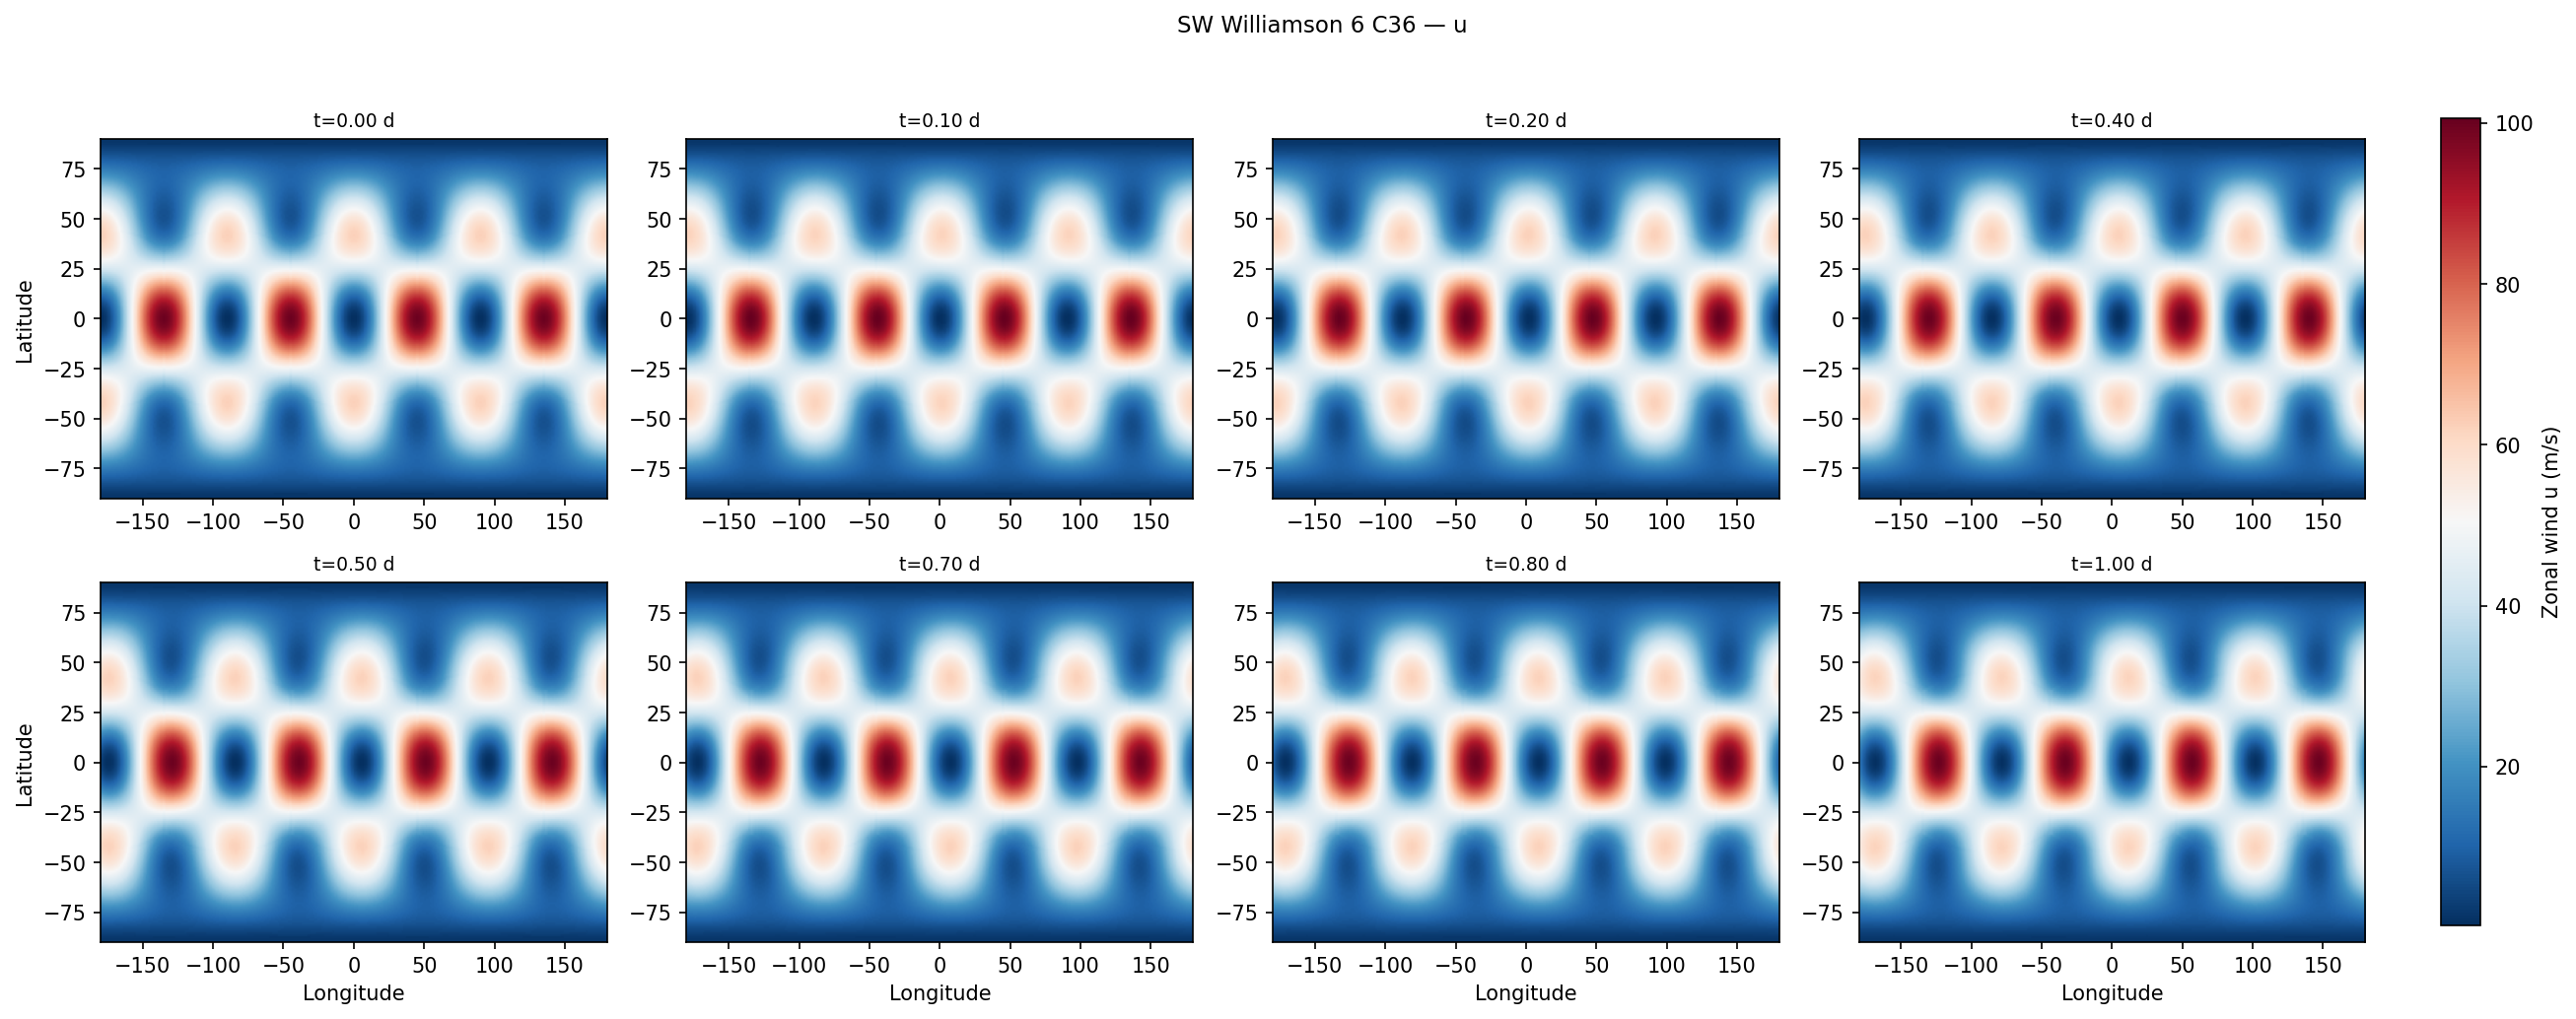
\includegraphics[width=\textwidth]{si_sw_w6_cube.png}
\caption{Williamson 6 (Rossby--Haurwitz wave)}\end{subfigure}
\caption{Shallow-water Williamson 5 and 6 tests on the cubed sphere (C36).}\label{si:w5w6}
\end{figure}

\begin{figure}[h]\centering
\begin{subfigure}{0.495\textwidth}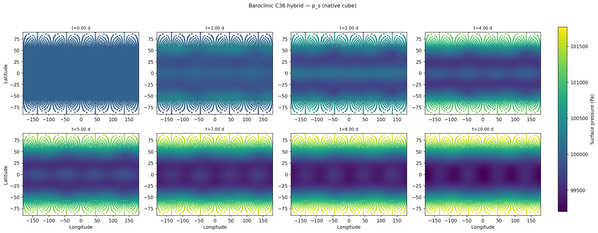
\includegraphics[width=\textwidth]{si_baroclinic_ps.jpg}
\caption{Surface pressure}\end{subfigure}\hfill
\begin{subfigure}{0.495\textwidth}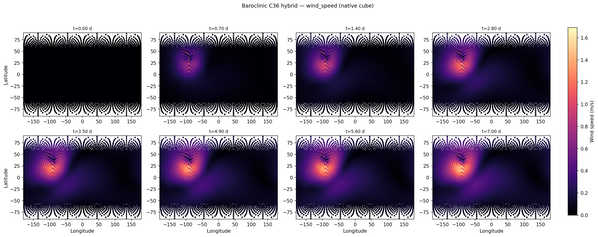
\includegraphics[width=\textwidth]{si_baroclinic_windspeed.jpg}
\caption{Wind speed}\end{subfigure}
\caption{Jablonowski--Williamson baroclinic-wave test, hydrostatic cubed-sphere C36, days
0--10. The instability grows at the expected rate and location.}\label{si:baroclinic}
\end{figure}

% #####################################################################
\section{Composability}
% #####################################################################
Composability operates on four orthogonal axes (main-text Fig.~1): grid, complexity, physics
and fidelity. Physics composition is additive to machine precision, $\texttt{tendency}(A+B+C)
=\texttt{tendency}(A)+\texttt{tendency}(B)+\texttt{tendency}(C)$, which is asserted by tests; a
process is disabled by setting its scheme to \texttt{"none"}, and every factory raises on an
unknown scheme rather than silently defaulting. An entire component can be swapped the same way:
in a short atmospheric integration the same slot accepts (i) the classical physics suite, (ii) a
column neural network, or (iii) a full SFNO dynamical core; and the ocean can be run as
prescribed SST, a slab mixed layer, or a full three-dimensional model from one driver. Table~S1
lists the dynamical cores; Tables~S2--S3 list the physics and ocean/land/ice schemes.

\begin{table}[h]\centering\footnotesize
\caption{Dynamical cores by equation set and discretization family.}\label{tab:cores}
\begin{tabular}{@{}lp{2.7cm}p{2.7cm}p{2.7cm}@{}}
\toprule
Discretization & Shallow water & Hydrostatic PE & Nonhydrostatic \\
\midrule
Cubed-sphere C-D (FV3) & \checkmark & \checkmark & \checkmark \\
Lat--lon C-grid (FV)   & \checkmark & \checkmark & -- \\
Gaussian/spectral      & \checkmark & \checkmark & \checkmark \\
Voronoi/MPAS (TRiSK)   & \checkmark & \checkmark & \checkmark \\
SFNO (learned)         & \checkmark & \checkmark & -- \\
Plane (LES/CRM)        & -- & -- & \checkmark \\
\bottomrule
\end{tabular}
\end{table}

\begin{table}[h]\centering\footnotesize
\caption{Atmospheric physics processes and representative schemes (each composable; set to
\texttt{none} to disable).}\label{tab:phys}
\begin{tabular}{@{}lp{10.5cm}@{}}
\toprule
Process & Schemes \\
\midrule
Radiation & gray (Frierson), RRTMGP correlated-$k$ (LW+SW), ML emulator \\
Convection & Bechtold, Tiedtke, Kain--Fritsch, Zhang--McFarlane, Emanuel, Kuo, unified mass-flux, EDMF, SBM, DCA \\
Microphysics & Kessler, Sundqvist, Morrison, Seifert--Beheng, Thompson, super-droplet, ML \\
Cloud fraction & Sundqvist, Xu--Randall \\
Boundary layer & Louis, Holtslag--Boville, YSU, EDMF, TKE 1.5, CLUBB-lite, Smagorinsky \\
Gravity-wave drag & Lindzen, Hines, McFarlane, Rayleigh, prognostic spectral, ML \\
\bottomrule
\end{tabular}
\end{table}

\begin{table}[h]\centering\footnotesize
\caption{Ocean, land and sea-ice schemes.}\label{tab:oli}
\begin{tabular}{@{}lp{10.5cm}@{}}
\toprule
Component & Schemes \\
\midrule
Ocean vertical mixing & KPP, Richardson, constant; Jayne--St-Laurent tidal \\
Ocean lateral mixing  & harmonic, biharmonic, GM--Redi, Visbeck, Leith, backscatter \\
Ocean grids           & lat--lon, Mercator, cubed-sphere C-D, MPAS Voronoi, tripolar (eORCA) \\
Land                  & slab (bucket); multi-layer Richards + Johansen thermal; DALEC carbon; snow \\
Sea ice               & thermodynamic slab; EVP/mEVP dynamic; multi-category ITD; ridging, ponds, brine \\
\bottomrule
\end{tabular}
\end{table}

% #####################################################################
\section{Multi-scale: large-eddy and cloud-resolving suites}
% #####################################################################
On a doubly periodic plane with the nonhydrostatic core and a scale-dependent dynamic
Smagorinsky closure, legoESM reproduces canonical LES cases: GABLS1\cite{Beare2006} (main-text
Fig.~4a), the Ekman layer, the Wangara diurnal cycle, and the DYCOMS-II\cite{Stevens2005} and
RICO\cite{vanZanten2011} cloud-topped boundary layers (Fig.~\ref{si:les}). Cloud-resolving
RCEMIP\cite{Wing2018} runs (Fig.~\ref{si:crm}) self-aggregate convection; warm-rain
microphysics matches a super-droplet Golovin coalescence benchmark\cite{Shima2009,Bartman2022}
(Fig.~\ref{si:sdm}). The Lagrangian super-droplet method (SDM) is supplied here as a
non-differentiable reference scheme rather than as a trainable component. Its particle-based
formulation is closely connected to what is measured in laboratory and field observations of
individual droplets, quantities that are otherwise very difficult to integrate at the global
modelling scale because of the scale mismatch, which makes it a valuable oracle for calibrating
the bulk schemes used in coarser configurations.

\begin{figure}[h]\centering
\begin{subfigure}{0.495\textwidth}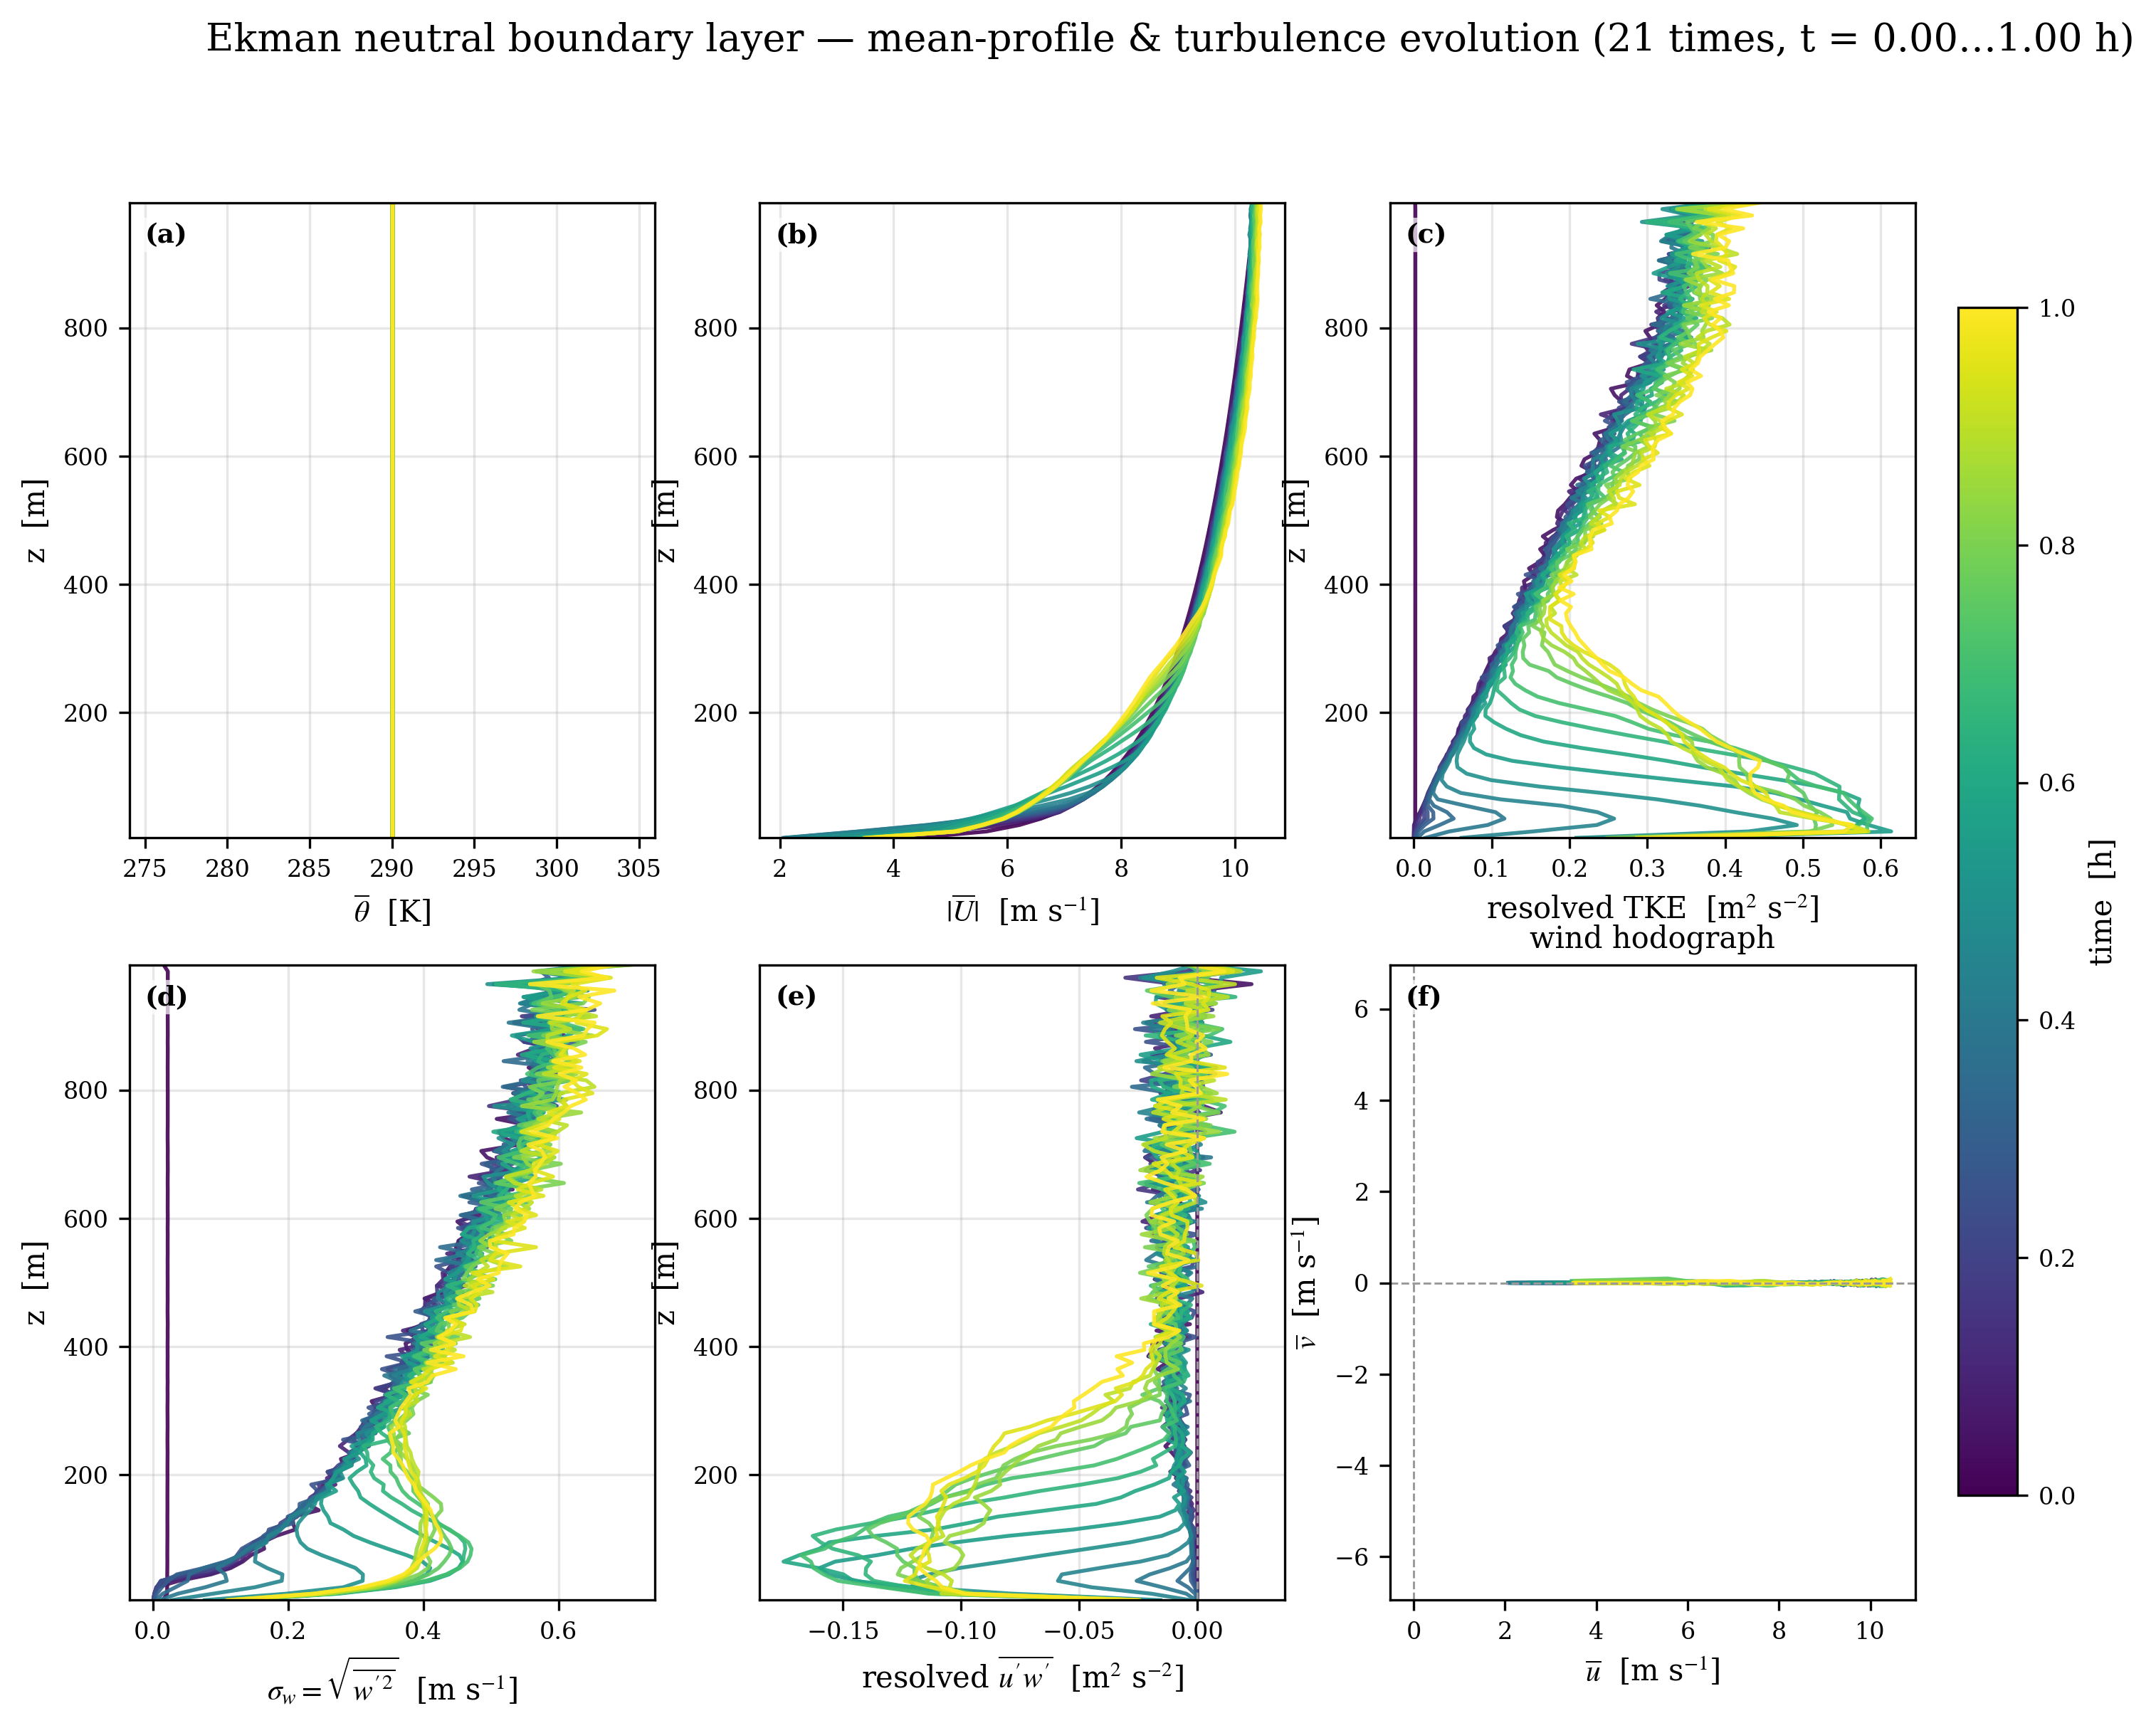
\includegraphics[width=\textwidth]{si_les_ekman.png}\caption{Ekman layer}\end{subfigure}\hfill
\begin{subfigure}{0.495\textwidth}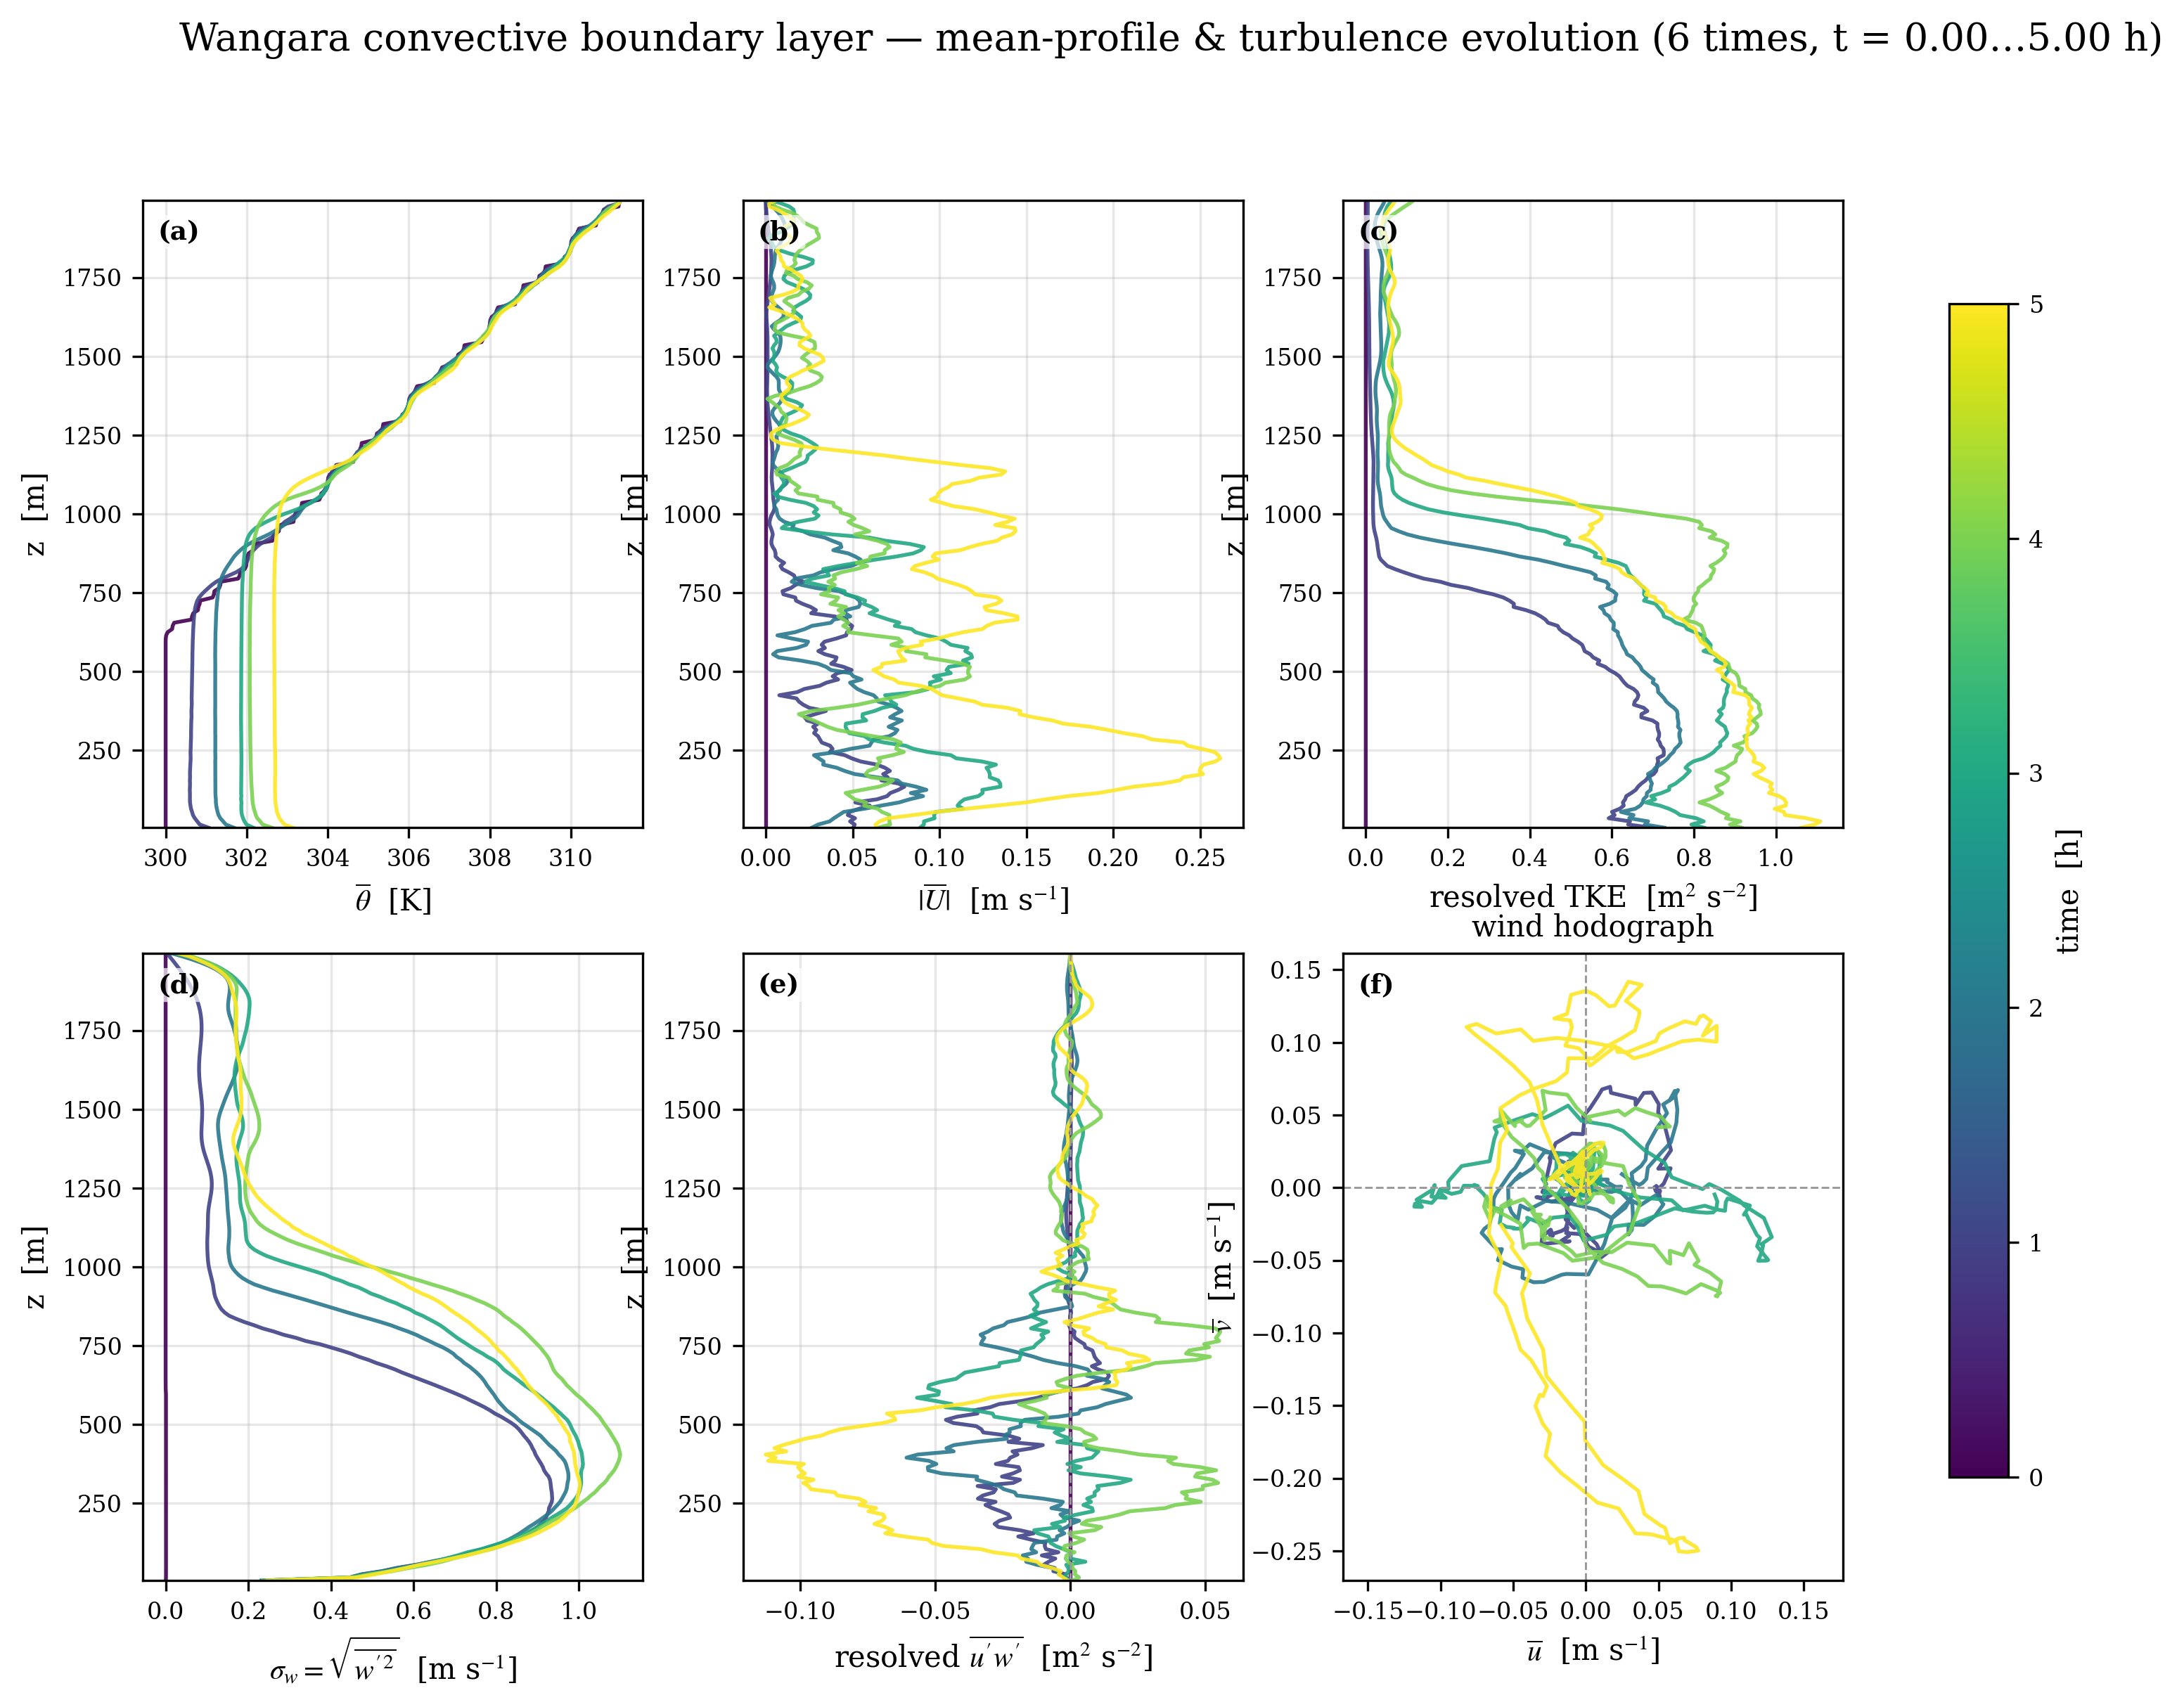
\includegraphics[width=\textwidth]{si_les_wangara.png}\caption{Wangara diurnal cycle}\end{subfigure}\\[3pt]
\begin{subfigure}{0.495\textwidth}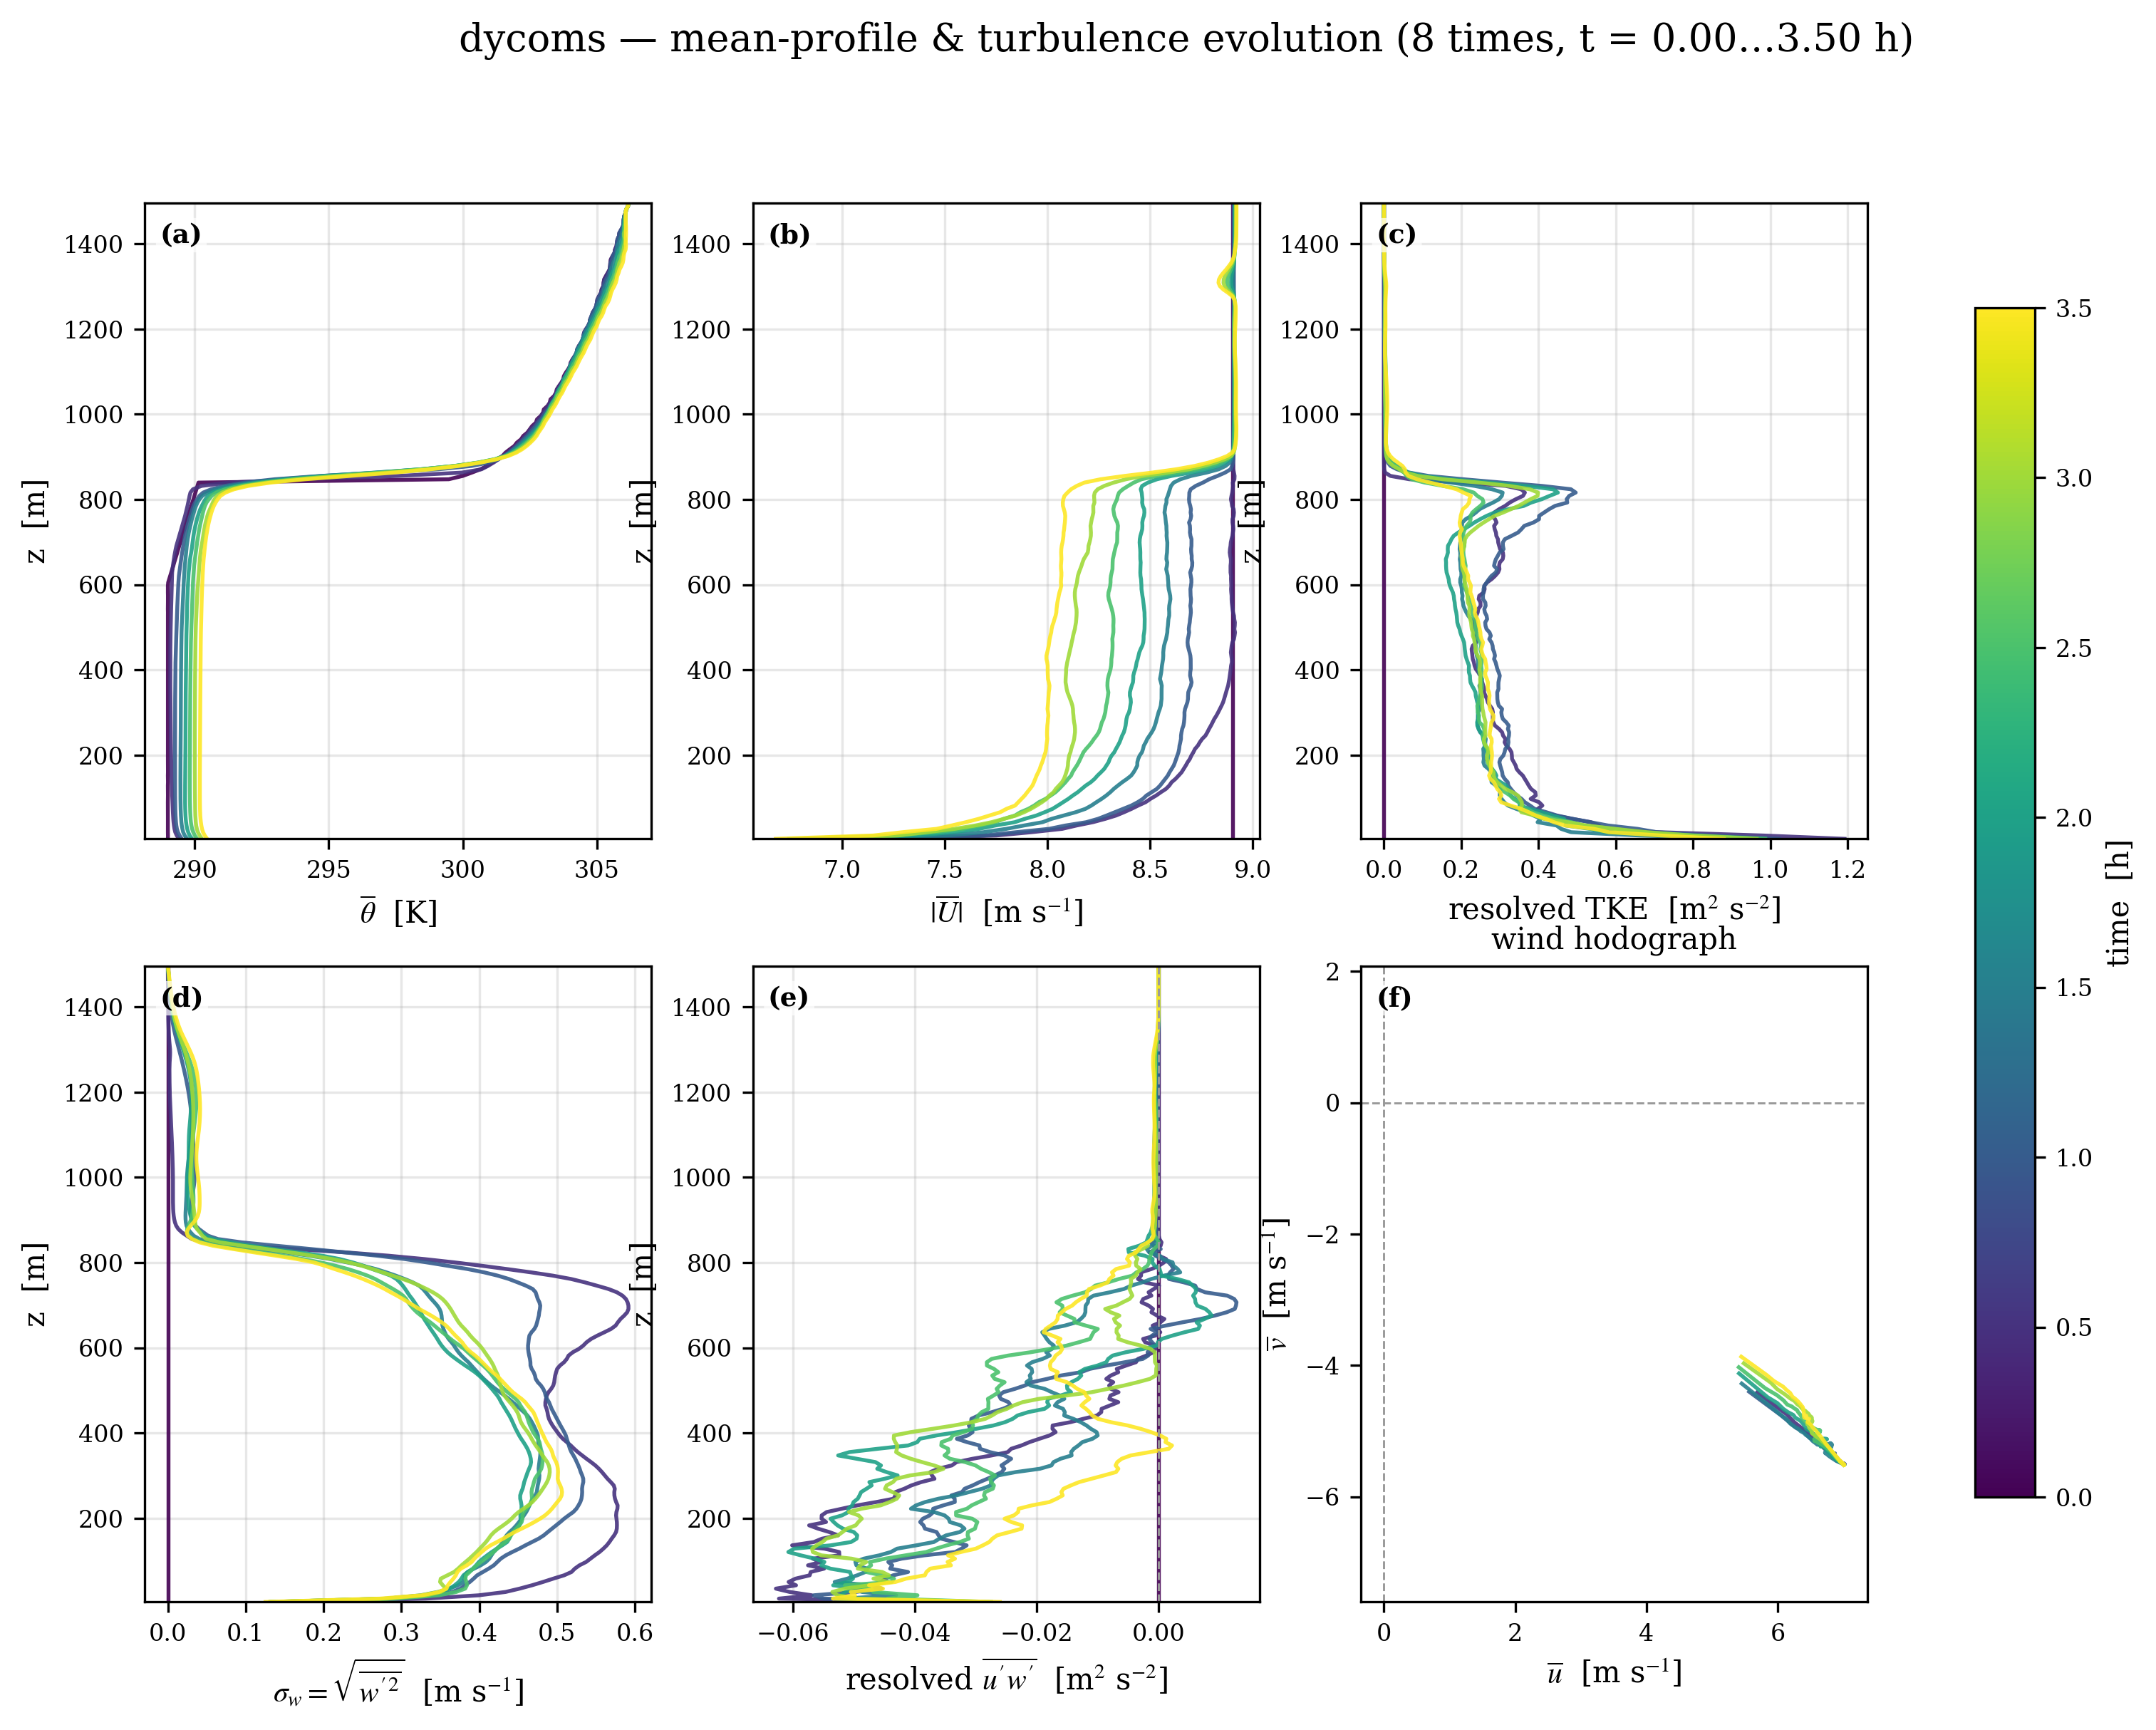
\includegraphics[width=\textwidth]{si_les_dycoms.png}\caption{DYCOMS-II stratocumulus}\end{subfigure}\hfill
\begin{subfigure}{0.495\textwidth}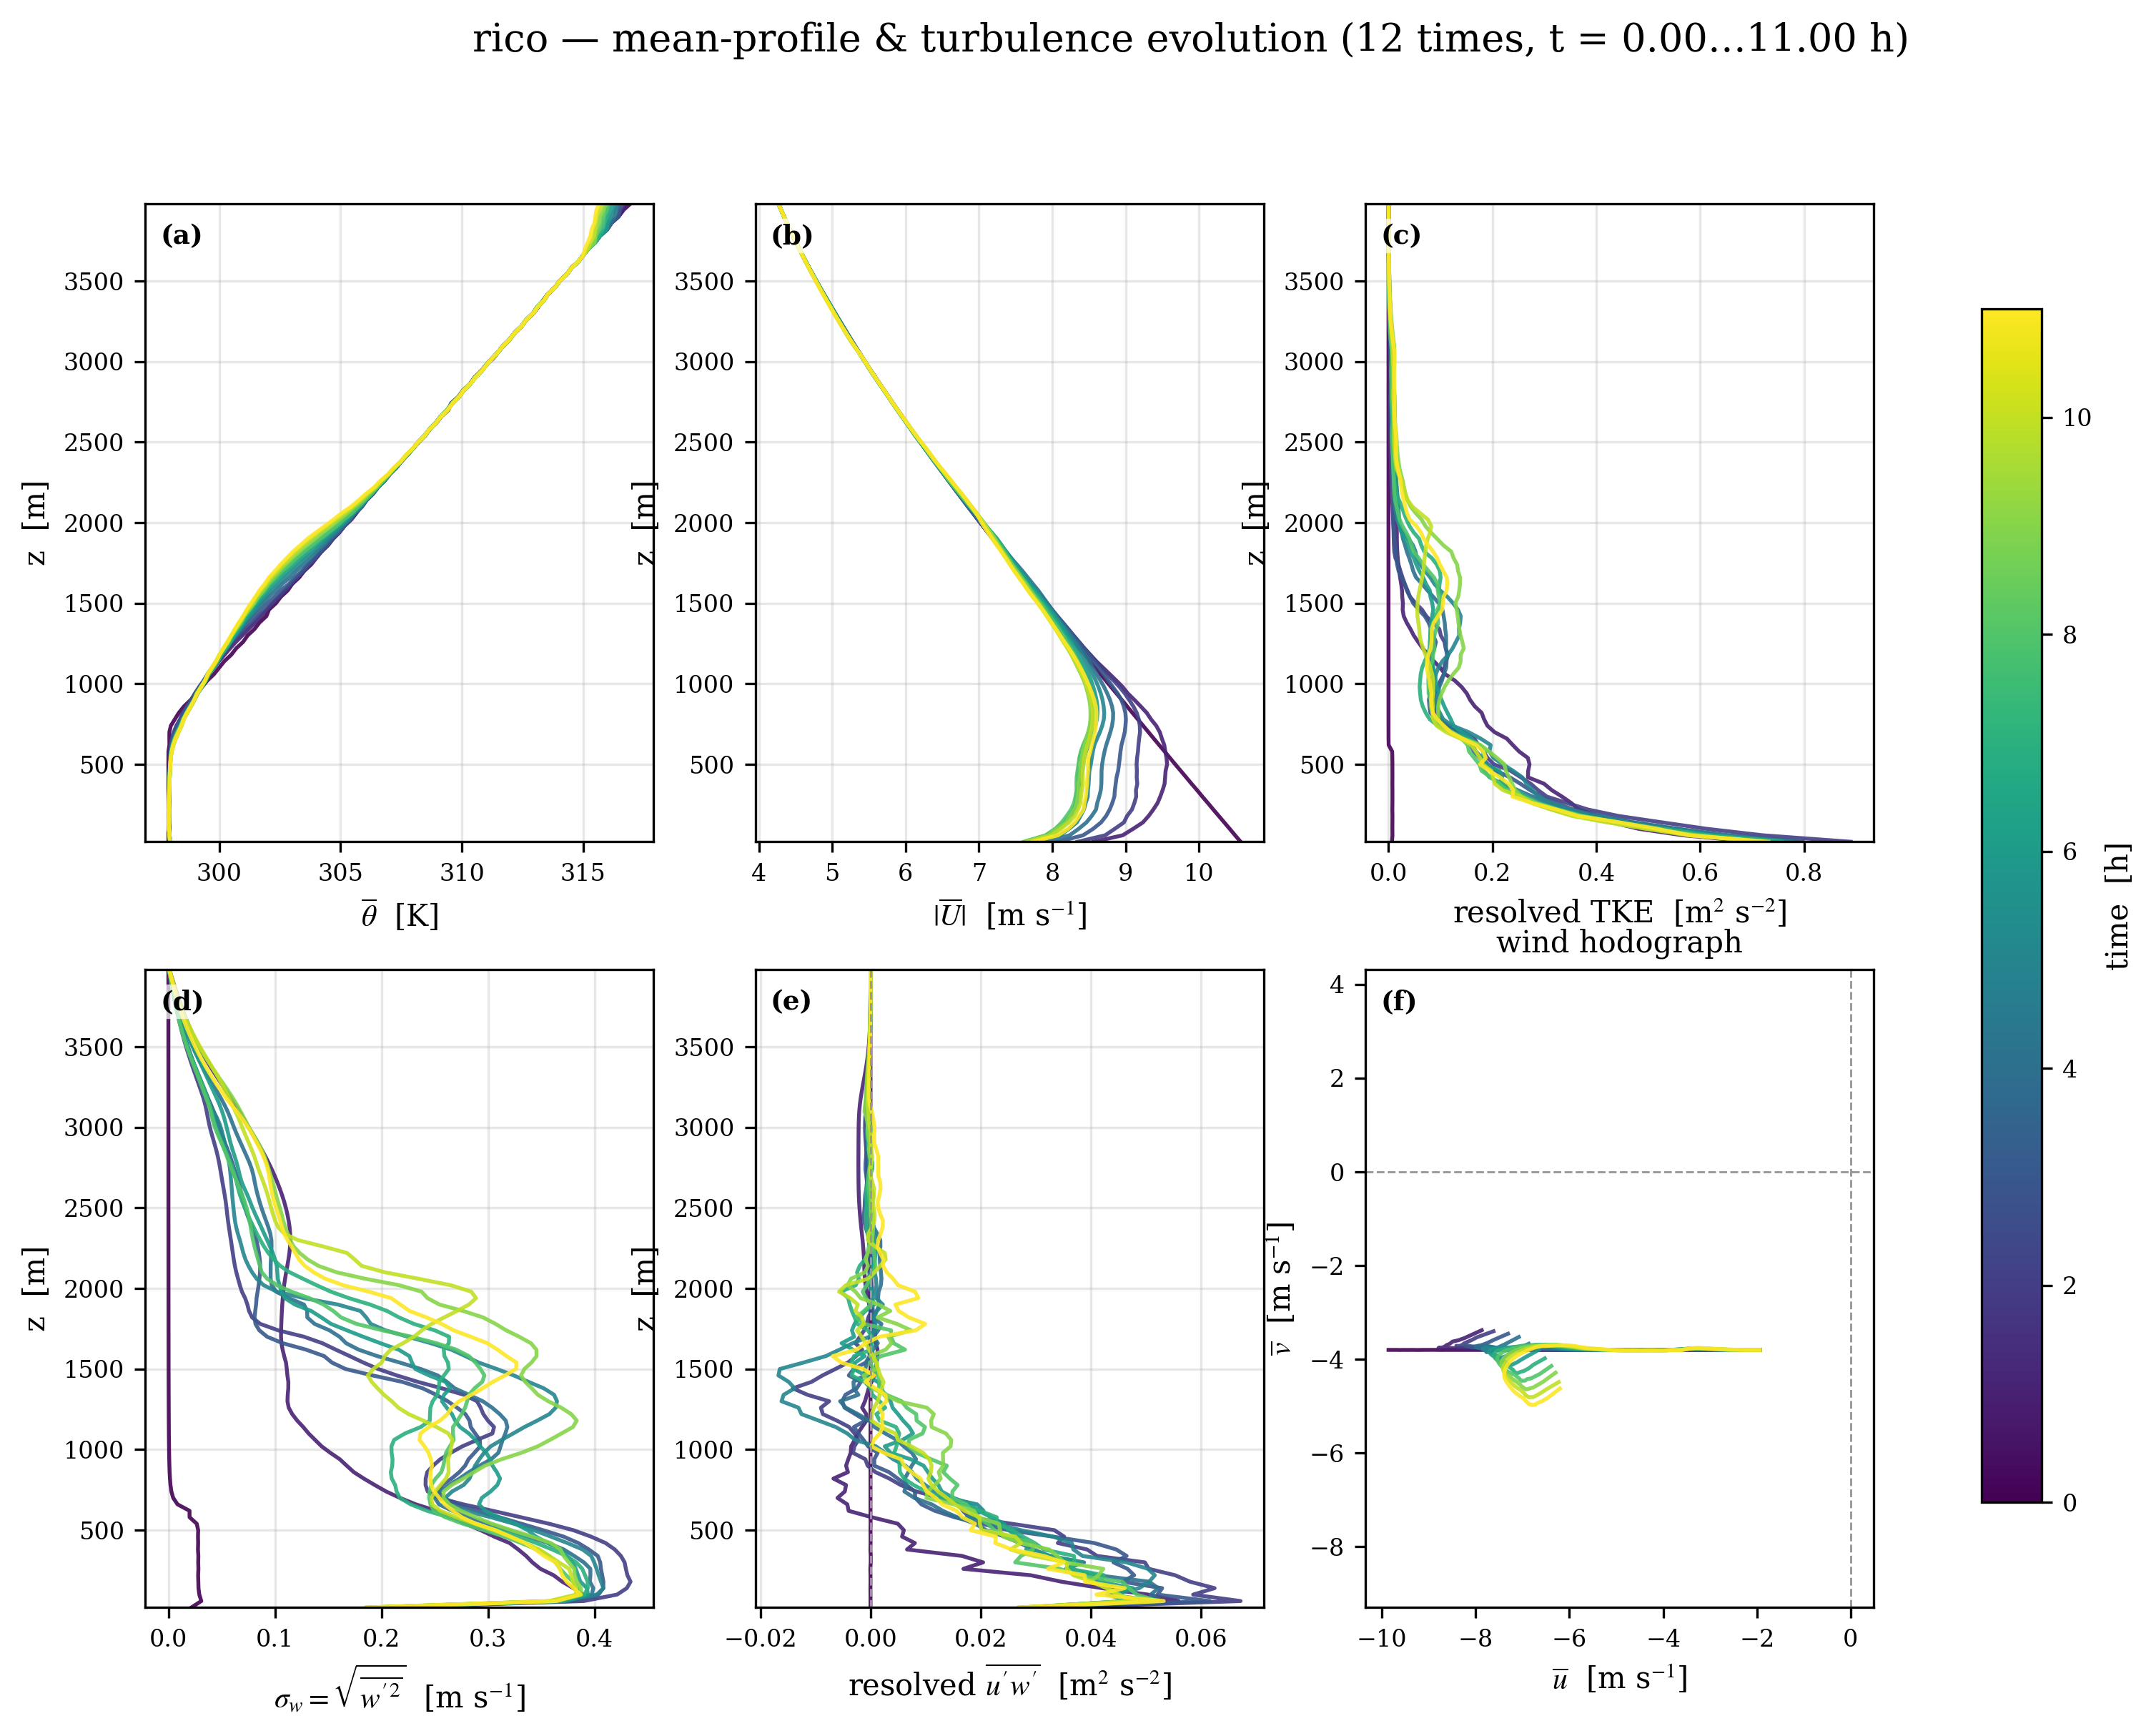
\includegraphics[width=\textwidth]{si_les_rico.png}\caption{RICO trade cumulus}\end{subfigure}
\caption{Large-eddy simulation of canonical boundary layers (profile evolution). Together with
GABLS1 (main-text Fig.~4a) these span stable, neutral, diurnal, stratocumulus and shallow-cumulus
regimes.}\label{si:les}
\end{figure}

\begin{figure}[h]\centering
\begin{subfigure}{0.62\textwidth}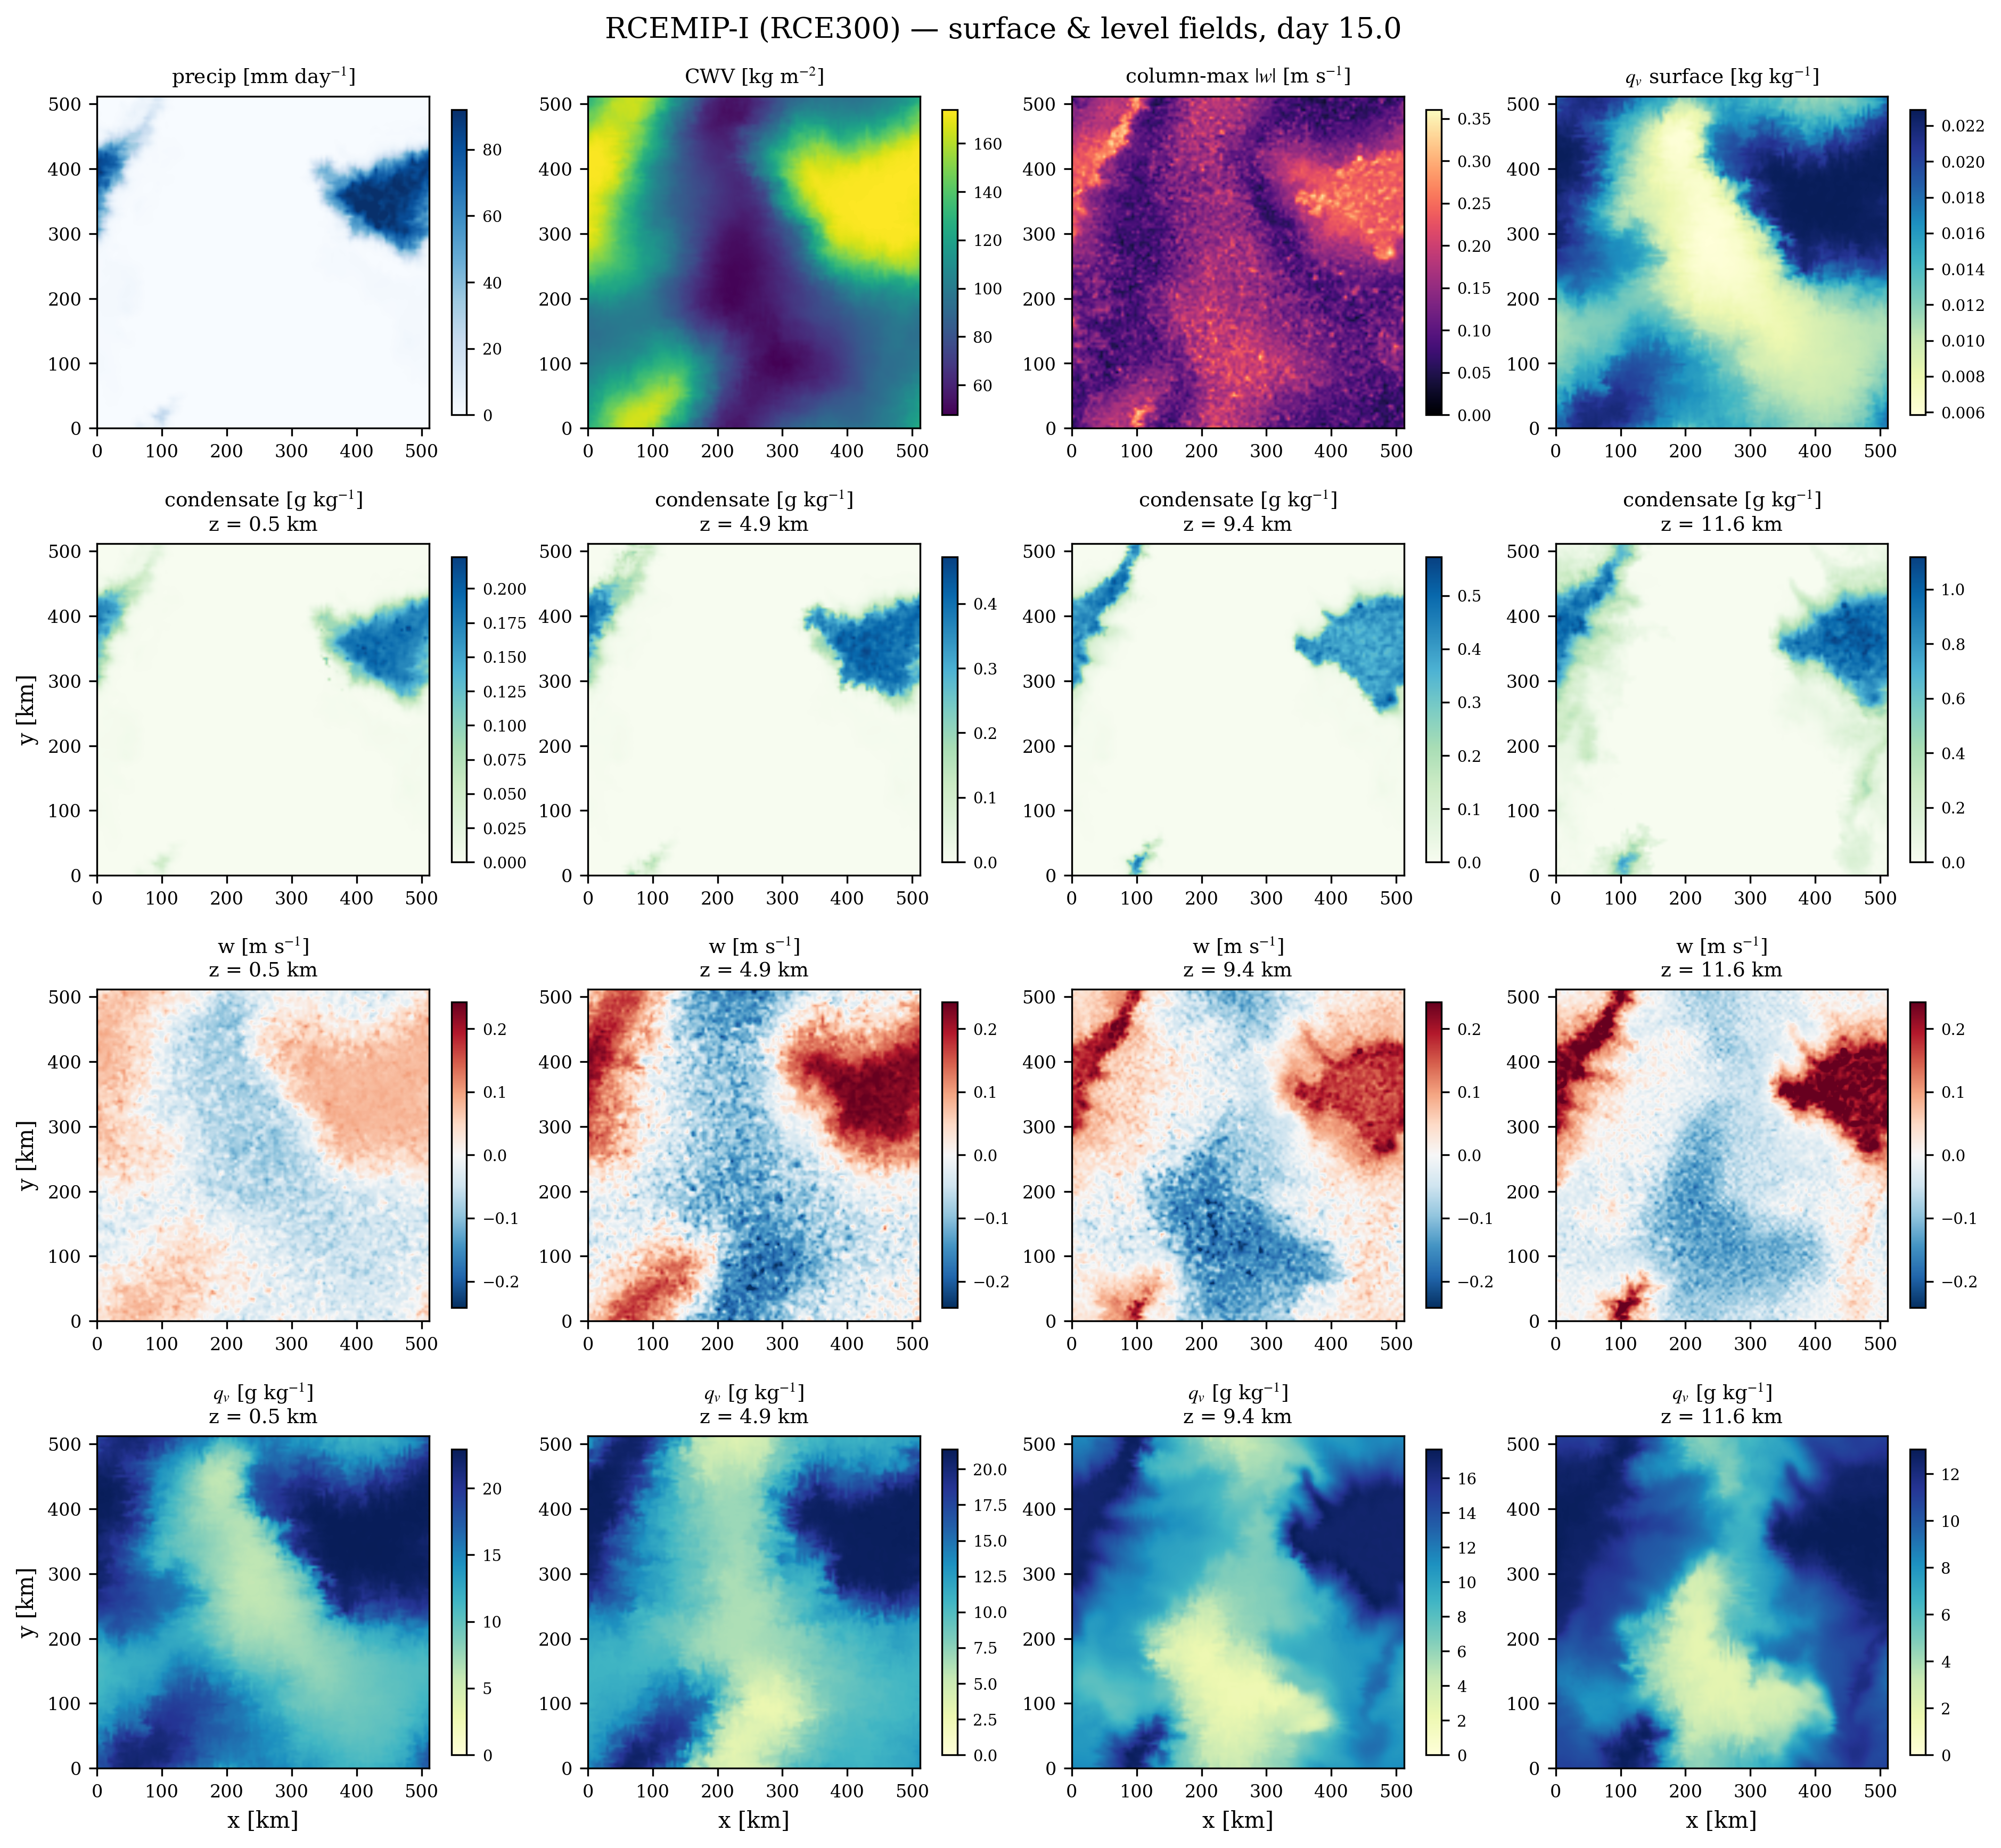
\includegraphics[width=\textwidth]{si_crm_rcemip2.png}\caption{RCEMIP surface/level fields}\end{subfigure}\hfill
\begin{subfigure}{0.36\textwidth}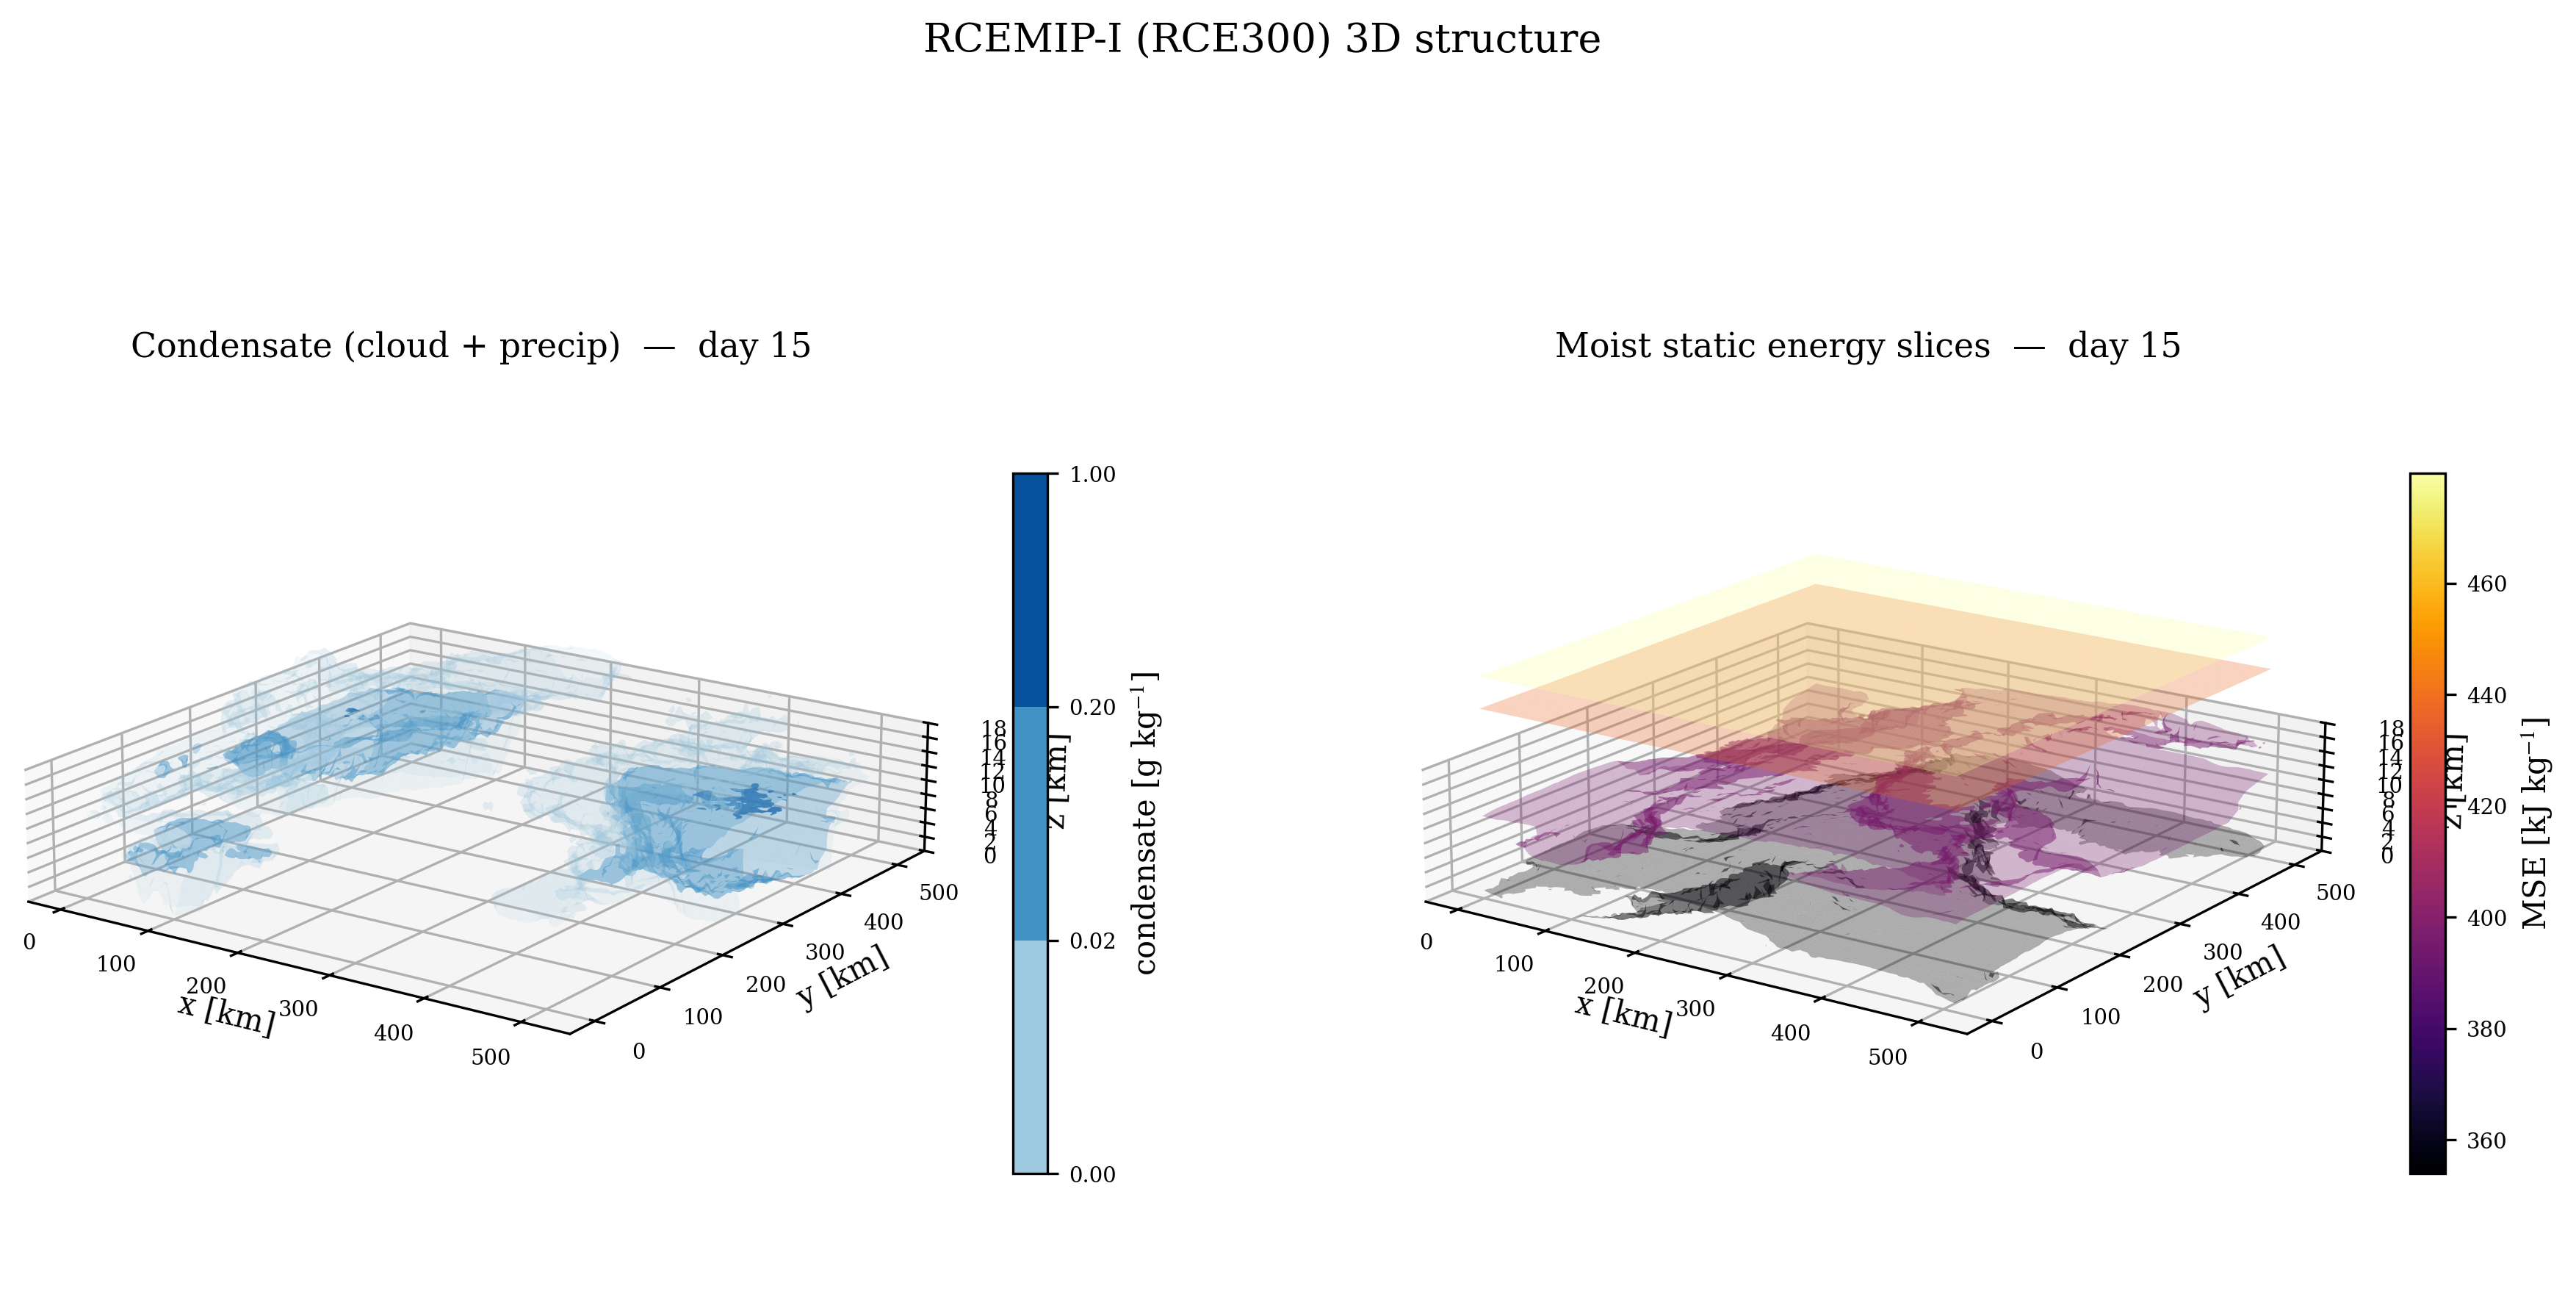
\includegraphics[width=\textwidth]{si_crm_vol3d.png}\caption{3D condensate}\end{subfigure}
\caption{Cloud-resolving RCE (RCEMIP RCE300): self-aggregated convection in surface/level fields
and a three-dimensional condensate snapshot.}\label{si:crm}
\end{figure}

\begin{figure}[h]\centering
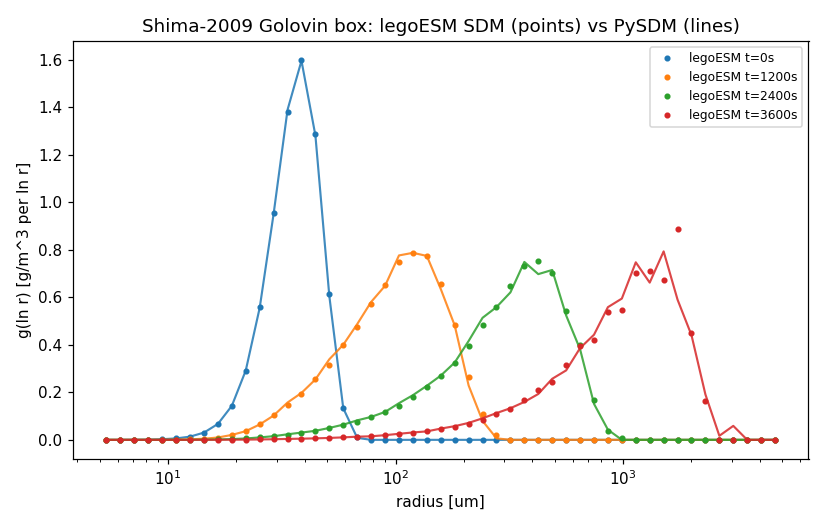
\includegraphics[width=0.7\textwidth]{si_microphysics_sdm.png}
\caption{Warm-rain collision--coalescence: legoESM bin/super-droplet microphysics vs.\ the PySDM
super-droplet reference on the Golovin analytic benchmark.}\label{si:sdm}
\end{figure}

% #####################################################################
\section{Ocean validation}
% #####################################################################
Beyond the main-text comparison (Fig.~5), Fig.~\ref{si:ocean} shows sea-surface salinity, mixed-layer
depth, a temperature--depth snapshot and a salinity section on the MPAS/Voronoi grid against
NEMO\cite{Madec2017}, and the MPAS sea-surface-height field. Figure~\ref{si:drake} shows a
multi-decadal Drake Passage spin-up: the zonal transport and zonal-mean zonal-velocity structure
equilibrate, demonstrating a stable Antarctic Circumpolar Current under the split-explicit solver.

\begin{figure}[h]\centering
\begin{subfigure}{0.495\textwidth}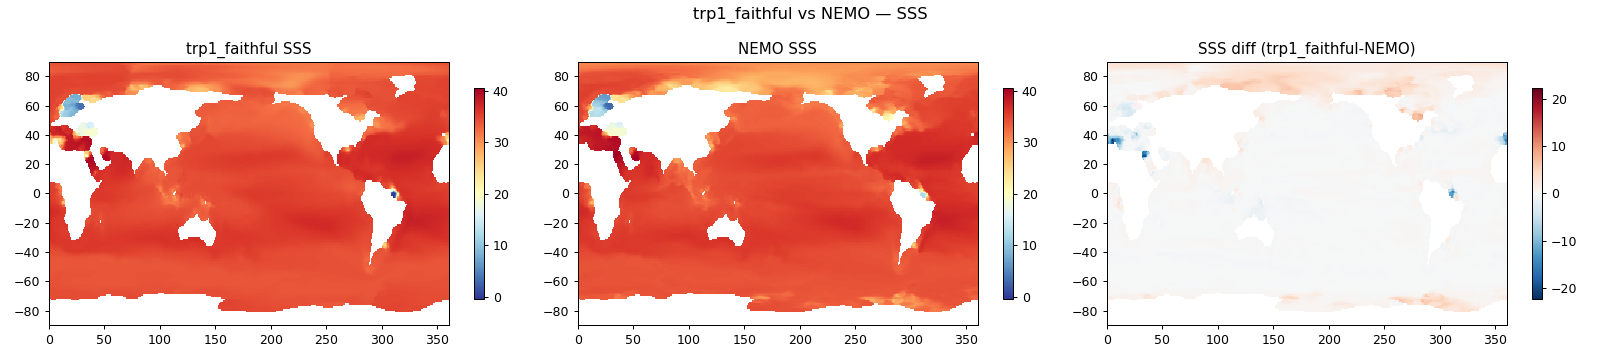
\includegraphics[width=\textwidth]{si_ocean_sss.png}\caption{Sea-surface salinity vs.\ NEMO}\end{subfigure}\hfill
\begin{subfigure}{0.495\textwidth}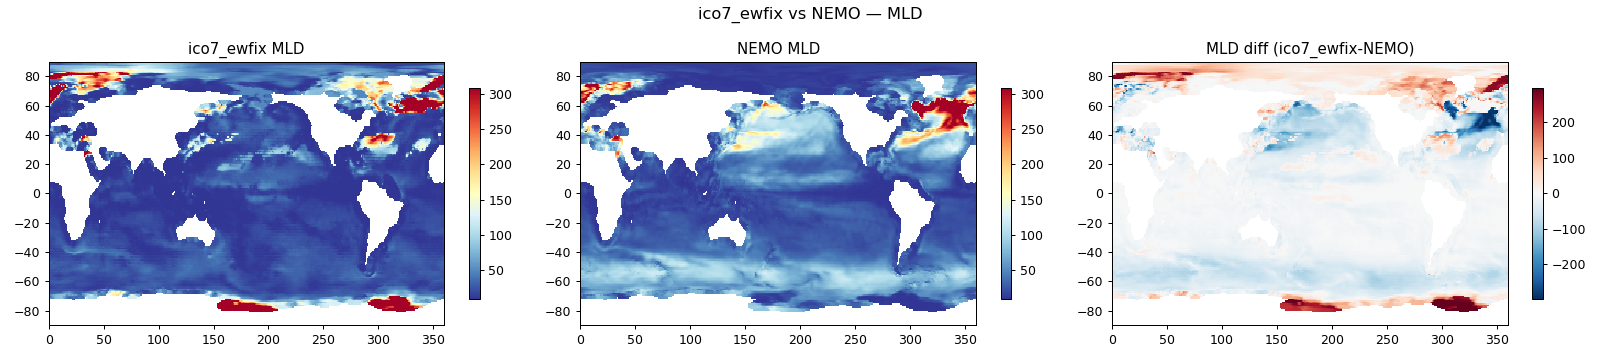
\includegraphics[width=\textwidth]{si_ocean_mld.png}\caption{Mixed-layer depth vs.\ NEMO}\end{subfigure}\\[3pt]
\begin{subfigure}{0.495\textwidth}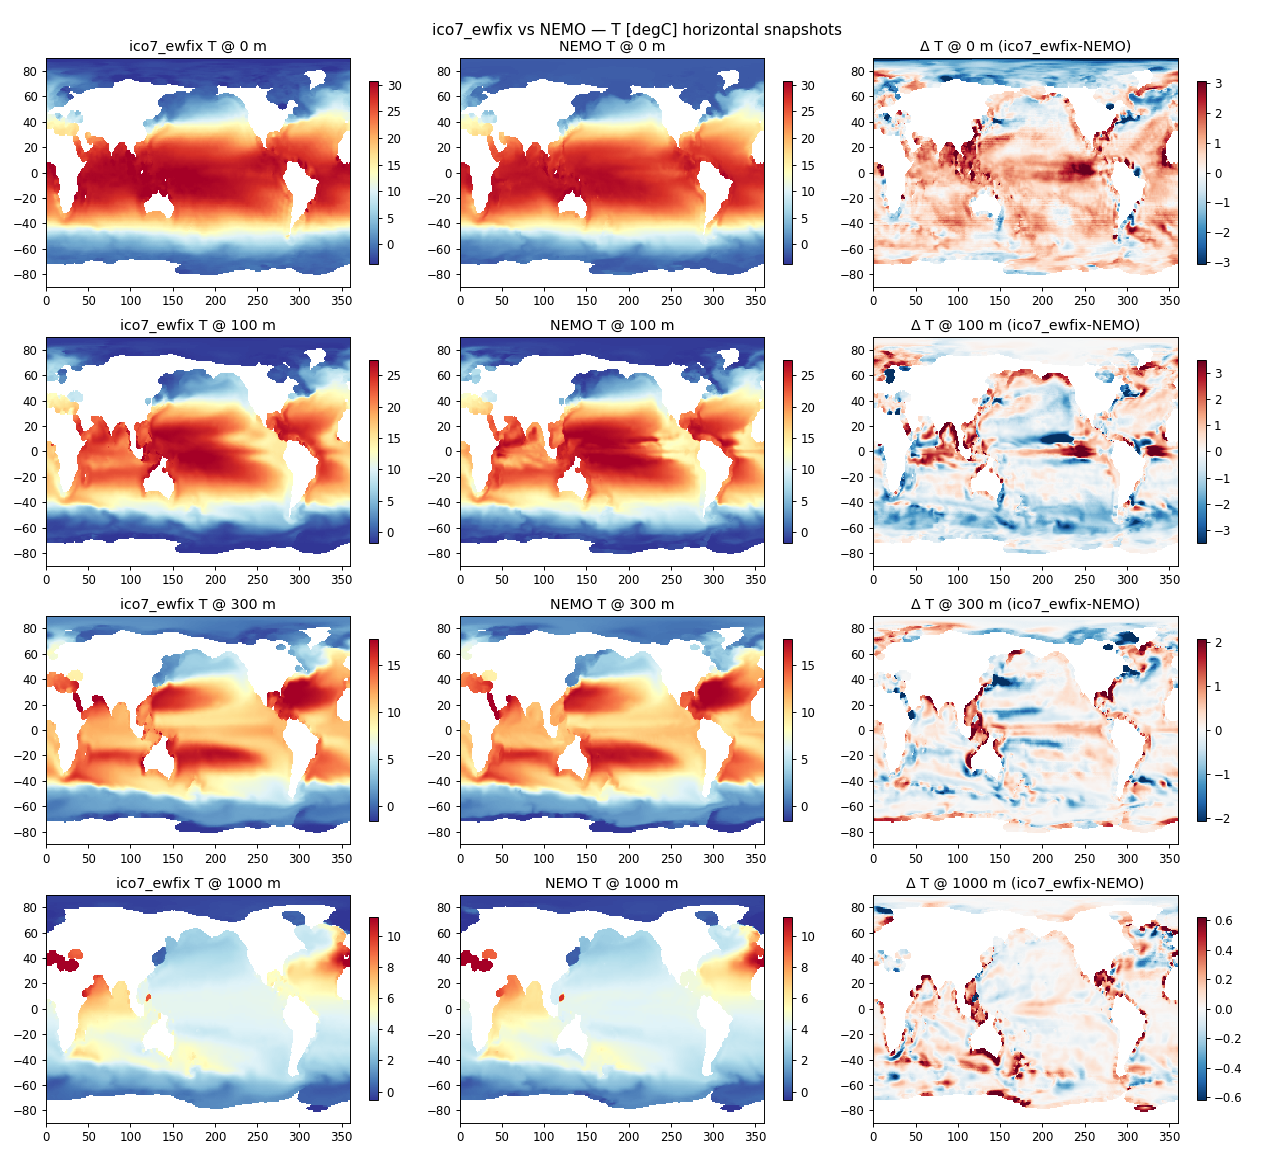
\includegraphics[width=\textwidth]{si_ocean_tdepth.png}\caption{Temperature at depth}\end{subfigure}\hfill
\begin{subfigure}{0.495\textwidth}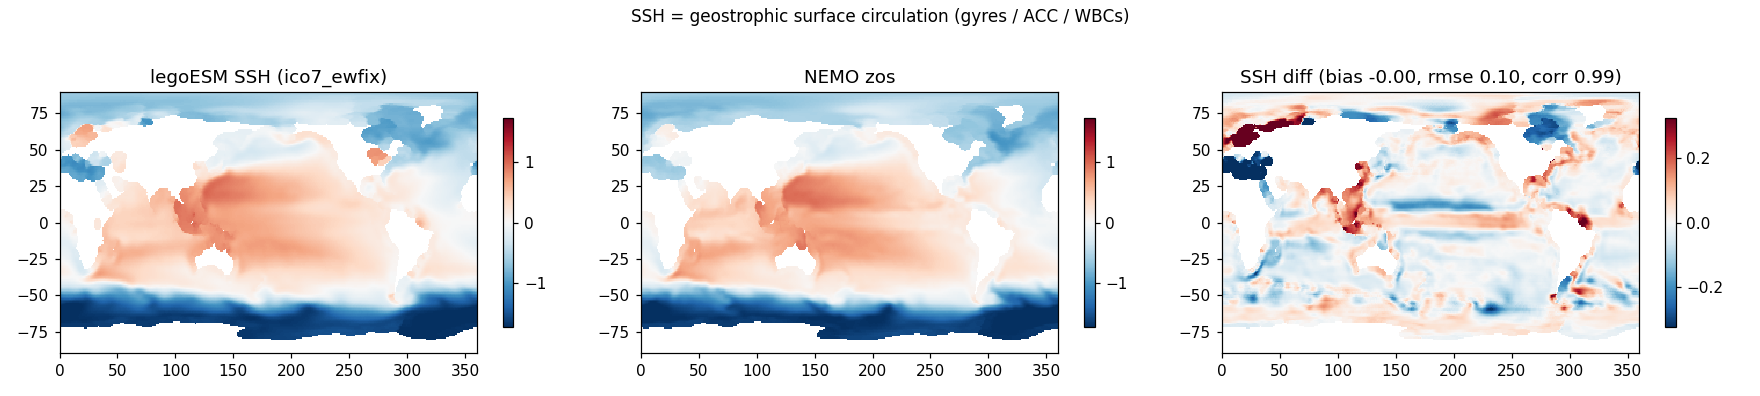
\includegraphics[width=\textwidth]{si_ocean_ssh_mpas.png}\caption{MPAS sea-surface height}\end{subfigure}
\caption{Additional MPAS/Voronoi ocean diagnostics against NEMO.}\label{si:ocean}
\end{figure}

\begin{figure}[h]\centering
\begin{subfigure}{0.495\textwidth}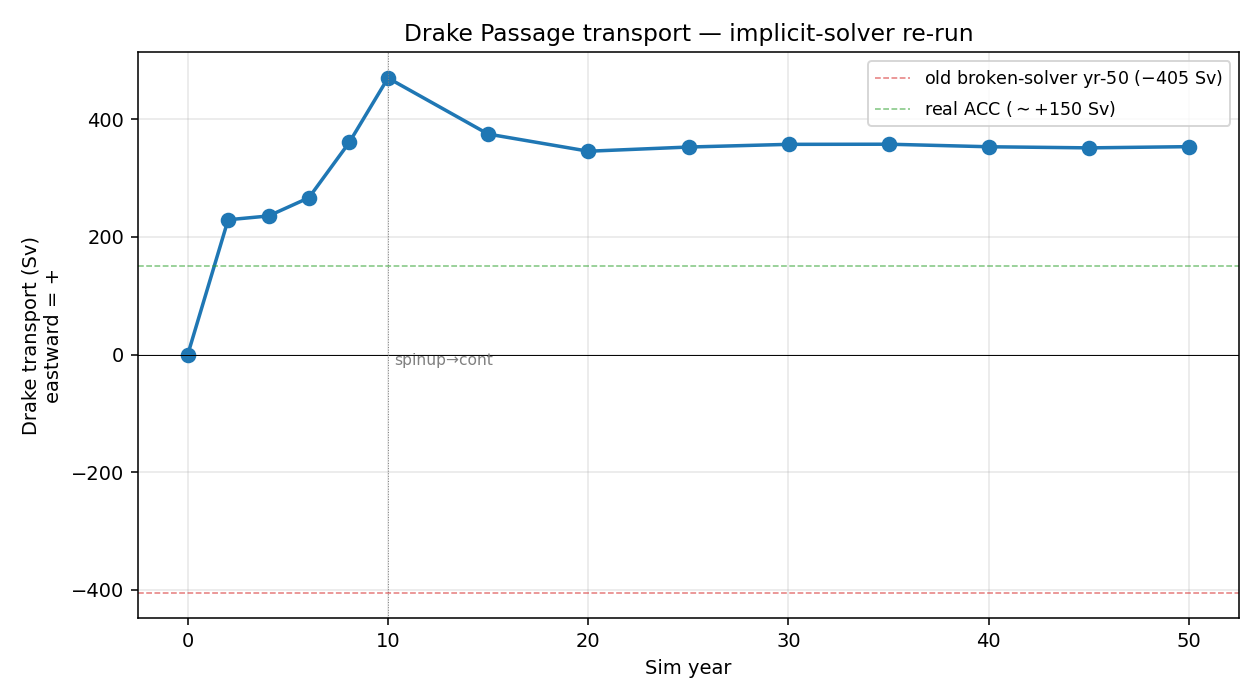
\includegraphics[width=\textwidth]{si_drake_transport.png}\caption{Drake Passage transport}\end{subfigure}\hfill
\begin{subfigure}{0.495\textwidth}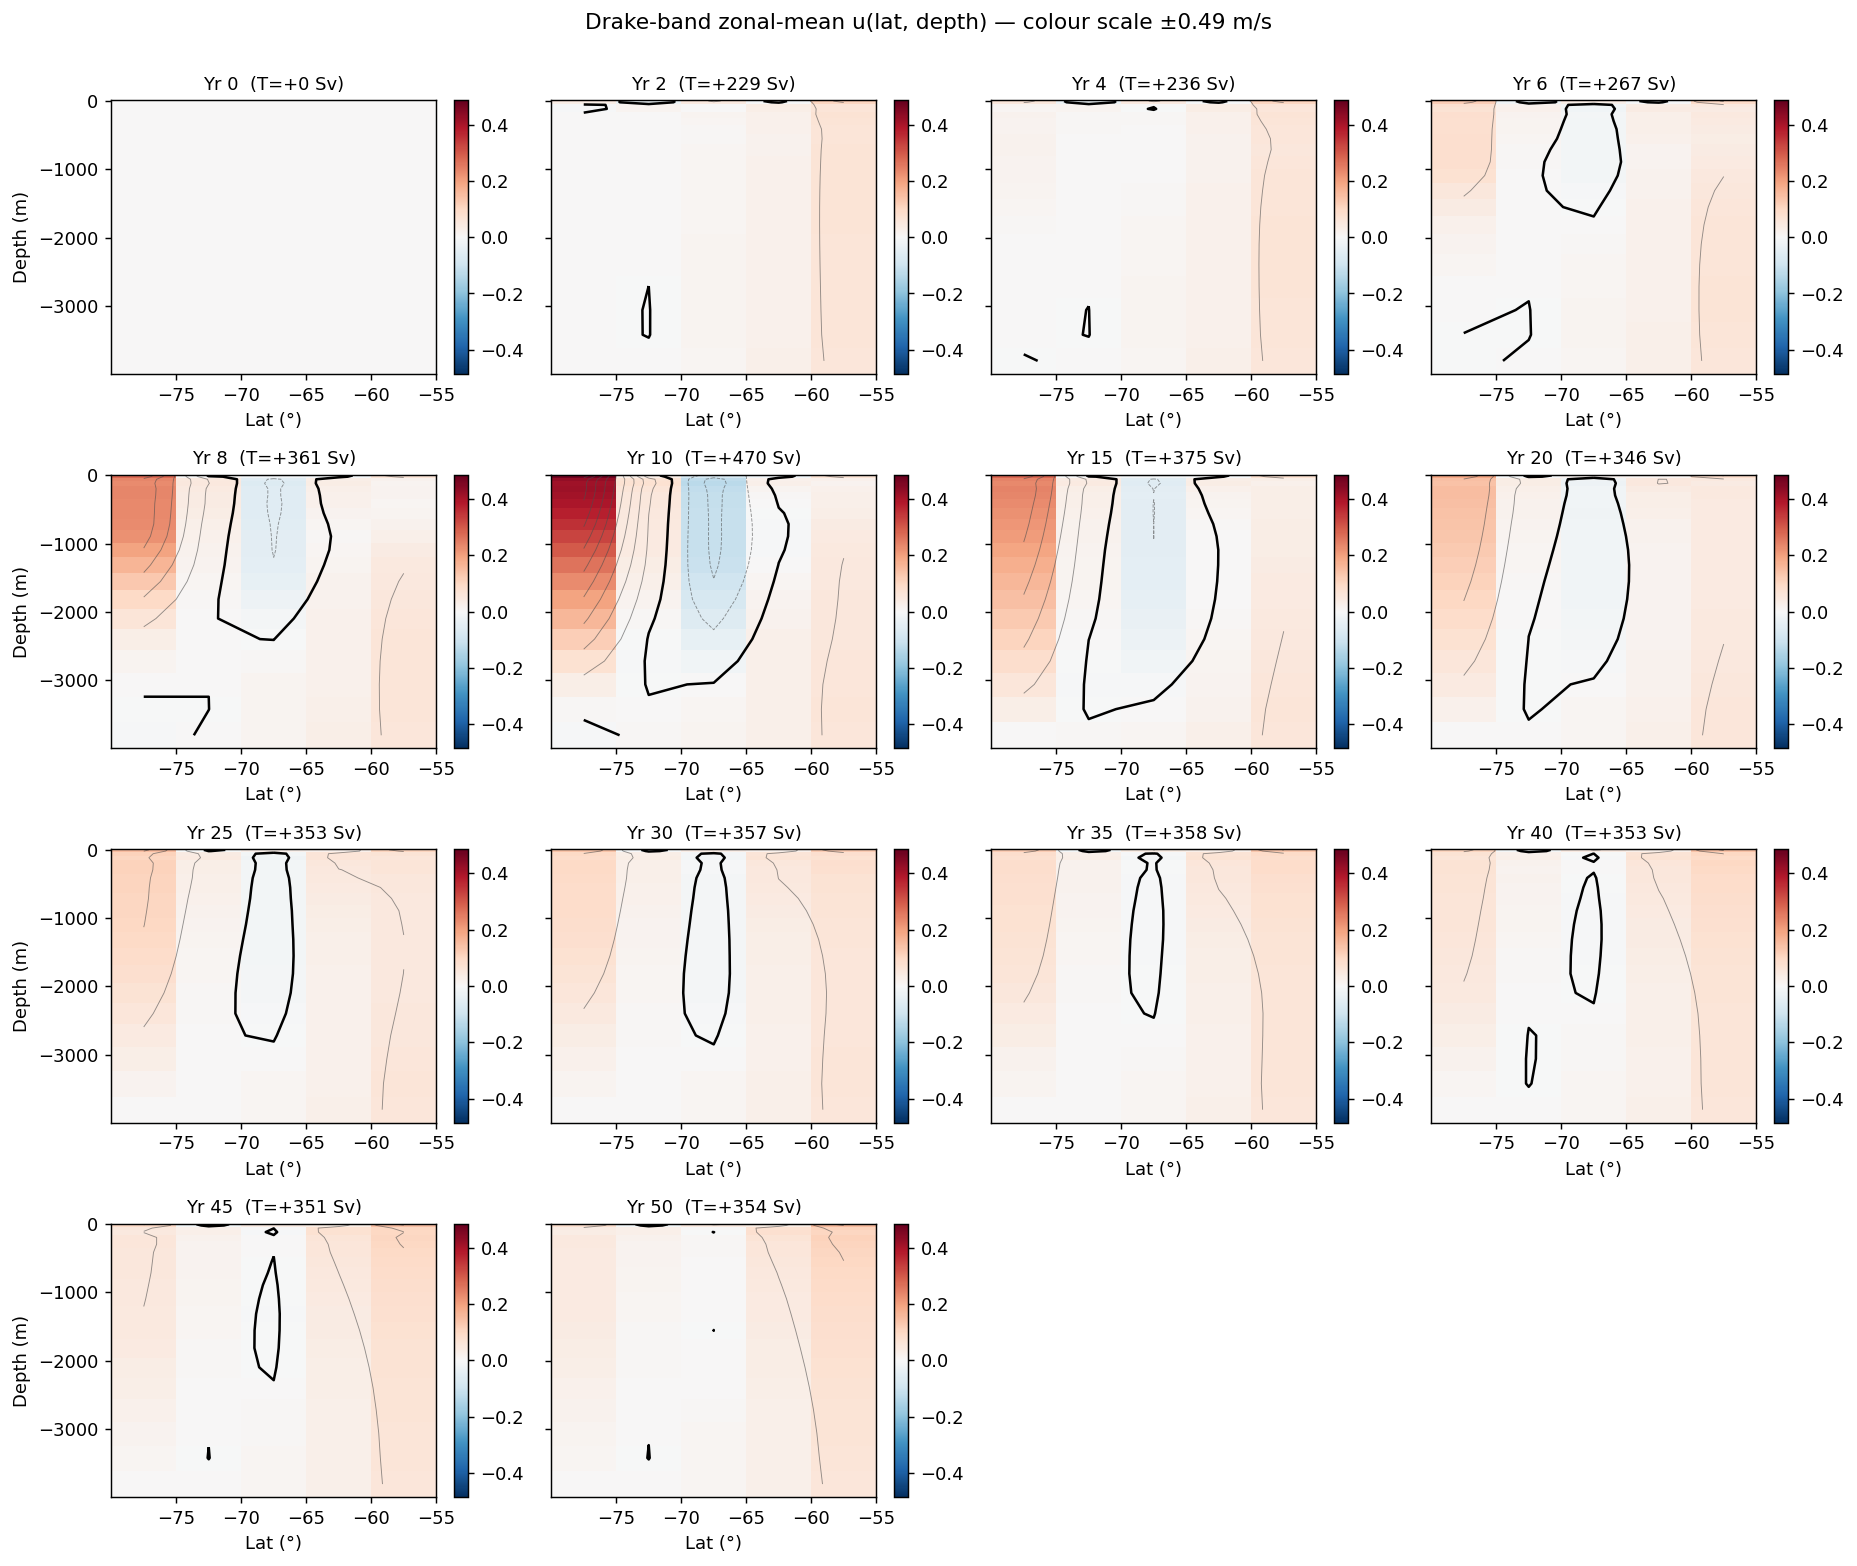
\includegraphics[width=\textwidth]{si_drake_u.png}\caption{Zonal-mean zonal velocity}\end{subfigure}
\caption{Multi-decadal Drake Passage / ACC spin-up showing a stable equilibrated circulation.}\label{si:drake}
\end{figure}

% #####################################################################
\section{Performance and scaling}
% #####################################################################
Throughput and acceleration numbers (Fig.~\ref{si:scaling}) were measured on a single RTX-class
GPU plus a 24-core CPU; strong/weak scaling was measured on a CPU cluster with one process per
node. Headline single-GPU throughput (Mcells\,s$^{-1}$, fp32) is 678 (lat--lon atmosphere), 404
(cubed-sphere), 298 (icosahedral), 400 (lat--lon ocean), 313 (tripolar) and 252 (MPAS ocean).
GPU acceleration over the CPU is $16$--$21\times$ (atmosphere) and $33$--$99\times$ (ocean) at fp32.
A halo-batching change (fewer, larger messages) improves the MPAS halo path (Fig.~\ref{si:halo}).

\begin{figure}[h]\centering
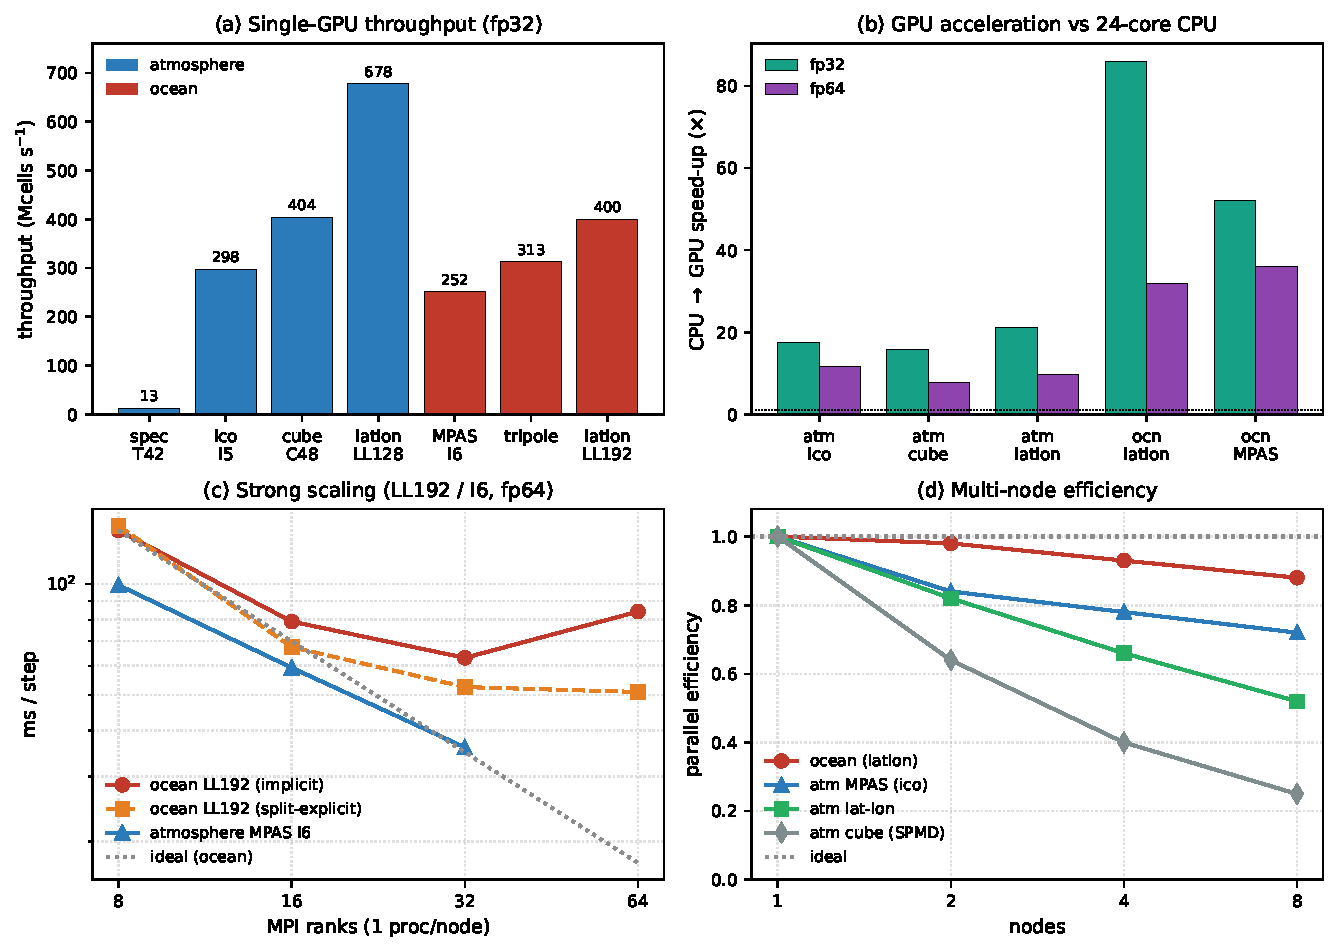
\includegraphics[width=0.96\textwidth]{f6_scaling.pdf}
\caption{\textbf{Portability and scaling.} (a) Single-GPU throughput (million cells per second,
fp32) across atmosphere and ocean grids. (b) CPU$\rightarrow$GPU speed-up at single and double
precision. (c) Strong scaling (time per step vs.\ MPI ranks; lower is better) for the ocean
(implicit vs.\ split-explicit barotropic solvers) and the MPAS atmosphere, against the ideal
line. (d) Multi-node parallel efficiency for the ocean and three atmospheric grids. All numbers
are measured on the hardware noted above.}\label{si:scaling}
\end{figure}
Reverse-mode differentiability is preserved across distributed execution: gradients through MPI
halo exchange (\texttt{sendrecv} with a custom adjoint) and \texttt{allreduce(SUM)} match
single-rank references to $\sim$$10^{-9}$. Documented limits: spectral transforms are
communication-bound on multi-GPU, and cross-node cubed-sphere panel exchange anti-scales on a
commodity TCP fabric (these are capability rather than speed-up results).

\begin{figure}[h]\centering
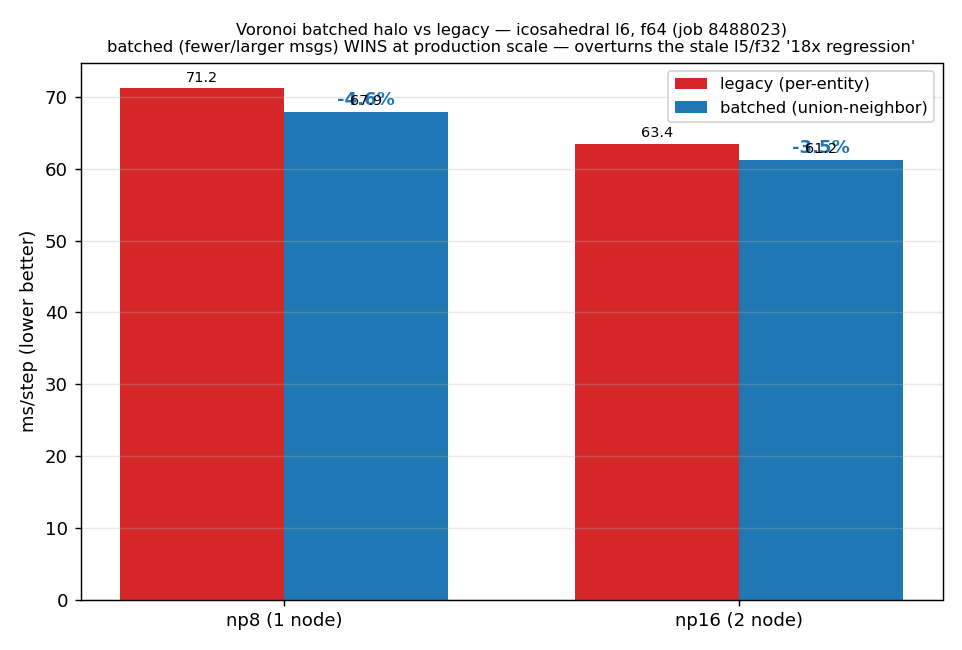
\includegraphics[width=0.7\textwidth]{si_scaling_halo.png}
\caption{Batched vs.\ legacy halo exchange on the MPAS/Voronoi grid (icosahedral level-6, fp64):
fewer/larger messages reduce time per step at 8 and 16 ranks.}\label{si:halo}
\end{figure}

% #####################################################################
\section{Accessibility: a worked example}
% #####################################################################
Because the model is idiomatic Python, configuring an experiment (here a single column with
gray radiation and a Louis boundary-layer scheme) is a few readable lines, and the same physics
object can be wrapped by a neural network or differentiated. This low barrier is a core design
goal for teaching and rapid prototyping.

\begin{lstlisting}
from legoesm.atmosphere.scm import SingleColumnModel
from legoesm.atmosphere.physics import PhysicsConfig, RadiationConfig, TurbulenceConfig
import jax.numpy as jnp

scm = SingleColumnModel.create(
    physics_config=PhysicsConfig(
        radiation=RadiationConfig(scheme="gray"),
        turbulence=TurbulenceConfig(scheme="louis")),
    nlev=40, dt=300.0,
    T_profile=jnp.linspace(220.0, 295.0, 40), latitude_deg=0.0)

final_state, history = scm.run(nsteps=288, save_every=12)   # 24 h at dt=300 s
\end{lstlisting}

\noindent Swapping \texttt{scheme="gray"} for \texttt{"rrtmgp"}, or \texttt{turbulence} for an
\texttt{"edmf"} or ML scheme, requires changing only the configuration; differentiating the run
with respect to any parameter requires wrapping \texttt{scm.run} in \texttt{jax.grad}.

% #####################################################################
\section{Physical consistency: operator-level tests}
% #####################################################################
Operators are verified against closed-form solutions (Fig.~\ref{si:phys}). The vector-invariant
advection reproduces the Burgers tendency $-u\,\pp_x u$; the Laplacian viscous term reproduces
$A_h\,\pp_{xx}u$ and its $k^2$ spectral scaling and exponential decay rate; the Coriolis term
gives $\dd v/\dd t=-fU$, $\dd u/\dd t=+fV$; and free inertial oscillations trace the analytic
hodograph. Under CFL-controlled refinement, finite-volume transport converges at its design order
and the semi-implicit gravity-wave solver at second order (Fig.~\ref{si:cfl}); documented gaps
(e.g.\ a parabolic-CFL regime where $\Delta t\propto\Delta x$) are reported rather than masked.

\begin{figure}[h]\centering
\begin{subfigure}{0.495\textwidth}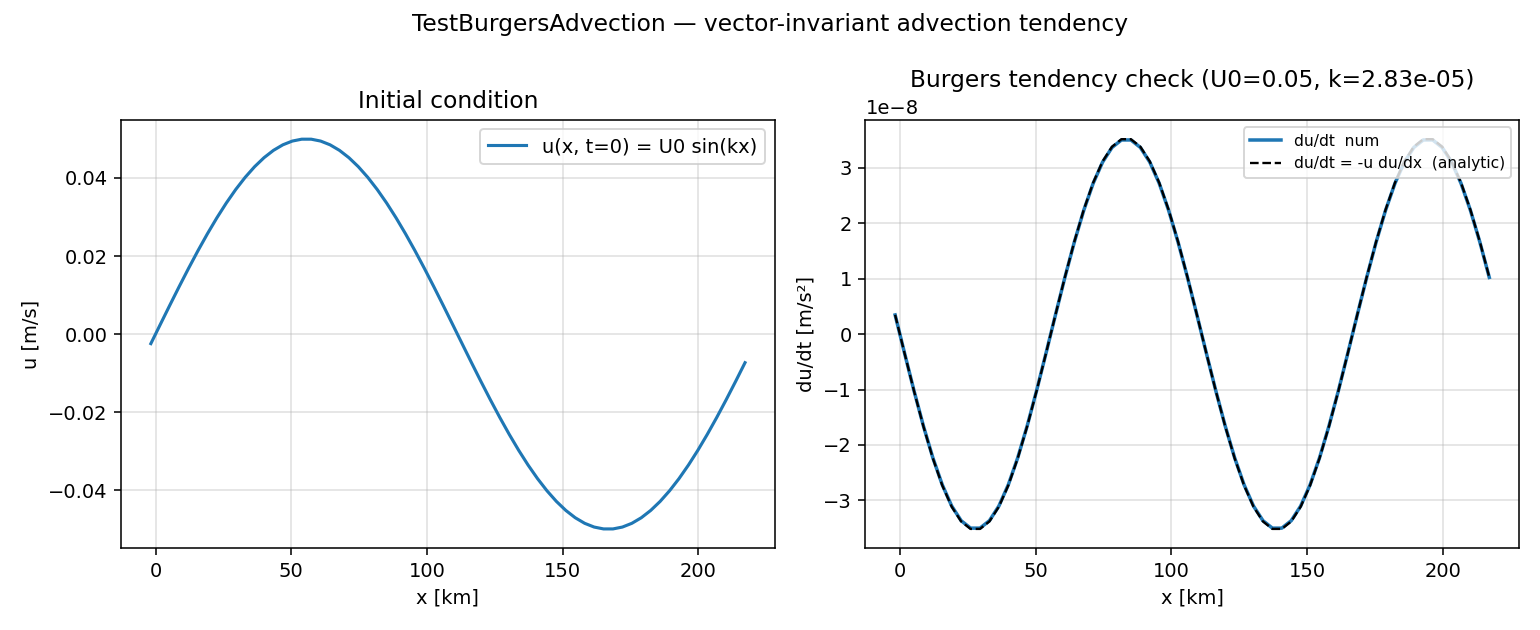
\includegraphics[width=\textwidth]{si_burgers.png}\caption{Vector-invariant (Burgers) advection}\end{subfigure}\hfill
\begin{subfigure}{0.495\textwidth}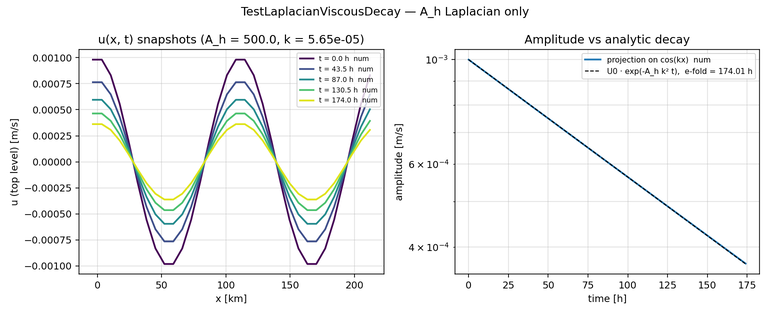
\includegraphics[width=\textwidth]{si_laplacian.png}\caption{Laplacian viscous, $k^2$ scaling}\end{subfigure}\\[3pt]
\begin{subfigure}{0.495\textwidth}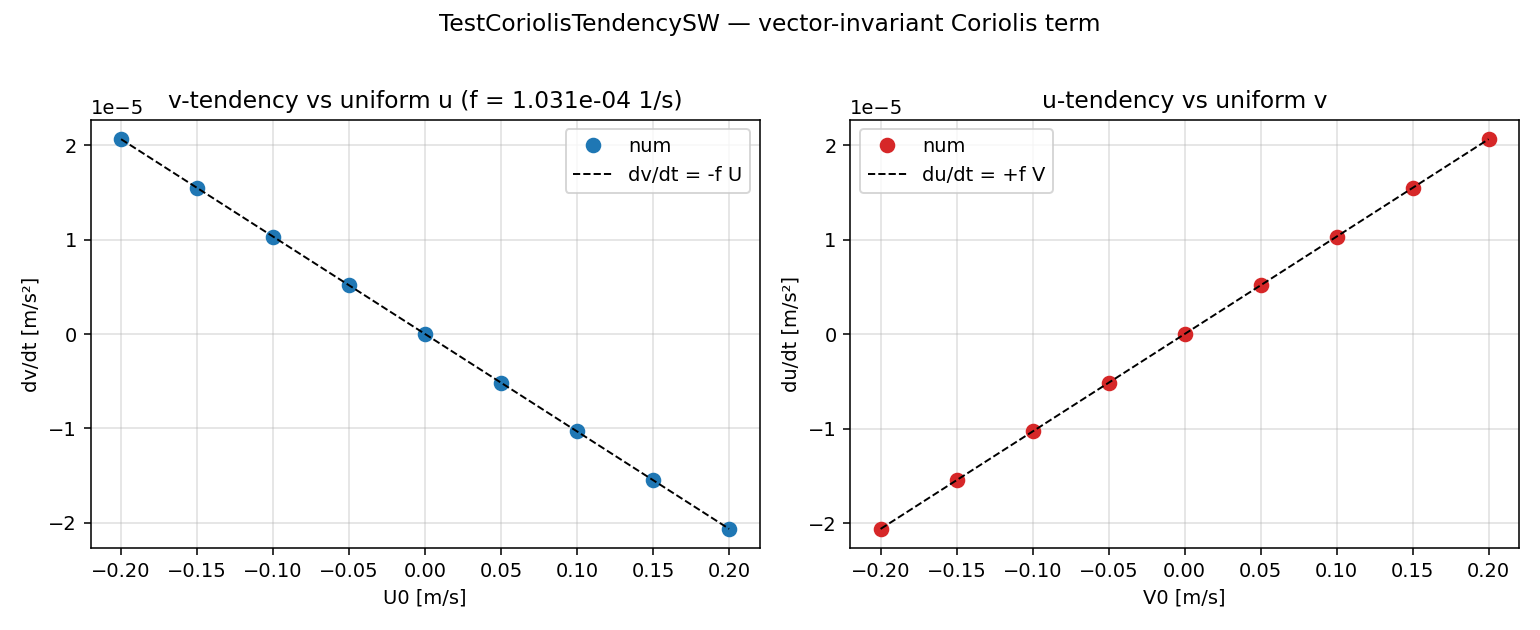
\includegraphics[width=\textwidth]{si_coriolis.png}\caption{Coriolis tendency}\end{subfigure}\hfill
\begin{subfigure}{0.495\textwidth}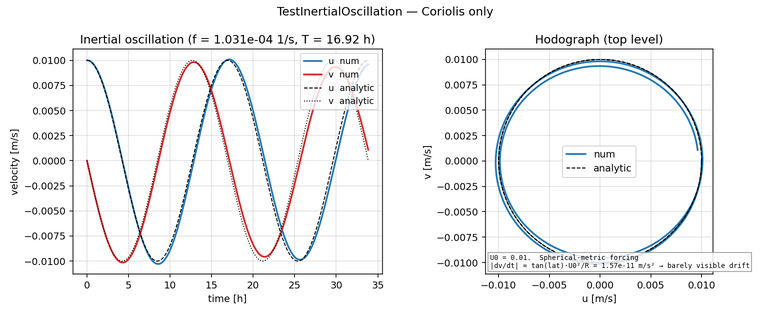
\includegraphics[width=\textwidth]{si_inertial.png}\caption{Inertial oscillation hodograph}\end{subfigure}
\caption{Operator tendencies (solid) against analytic solutions (dashed).}\label{si:phys}
\end{figure}

\begin{figure}[h]\centering
\begin{subfigure}{0.495\textwidth}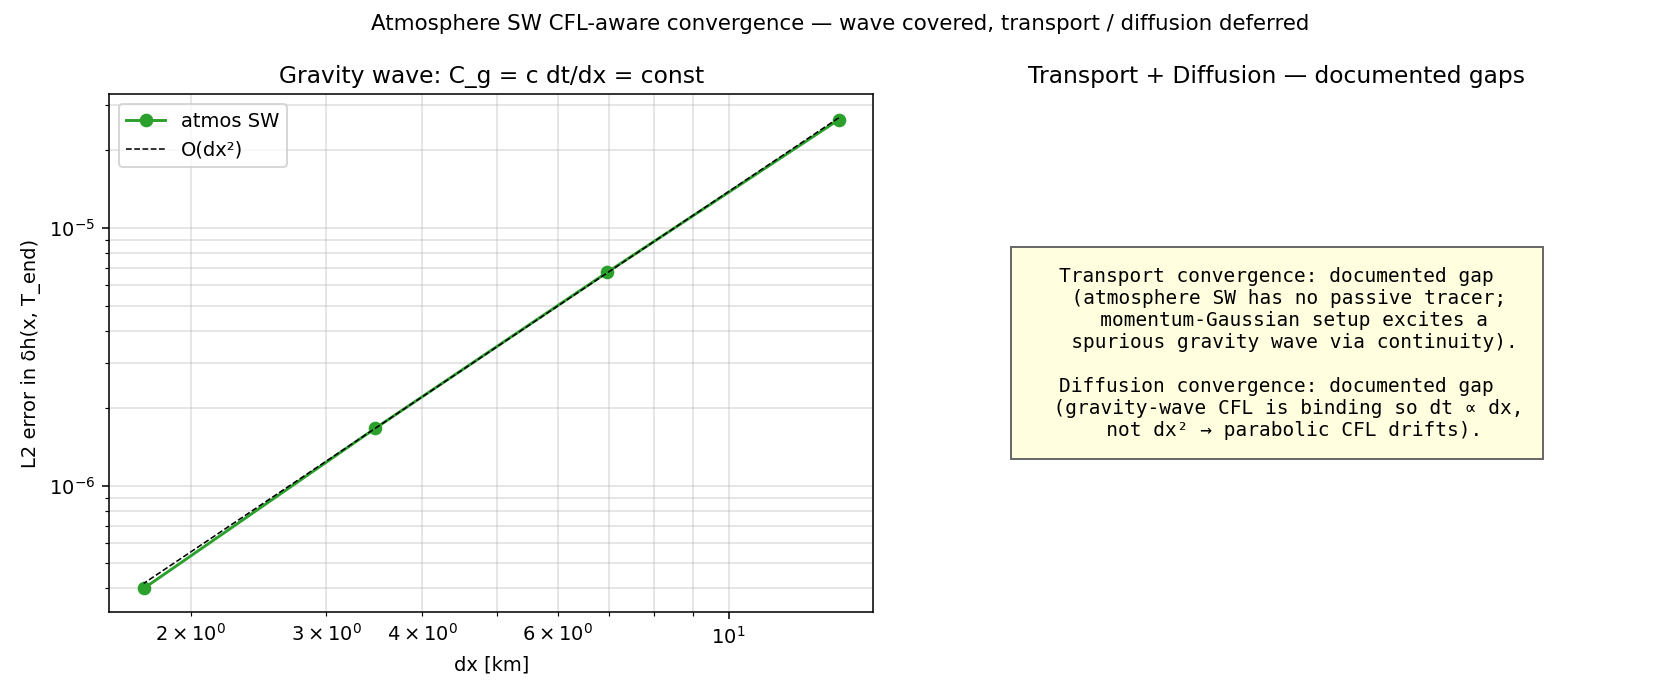
\includegraphics[width=\textwidth]{si_cfl_atm.png}\caption{Atmosphere SW}\end{subfigure}\hfill
\begin{subfigure}{0.495\textwidth}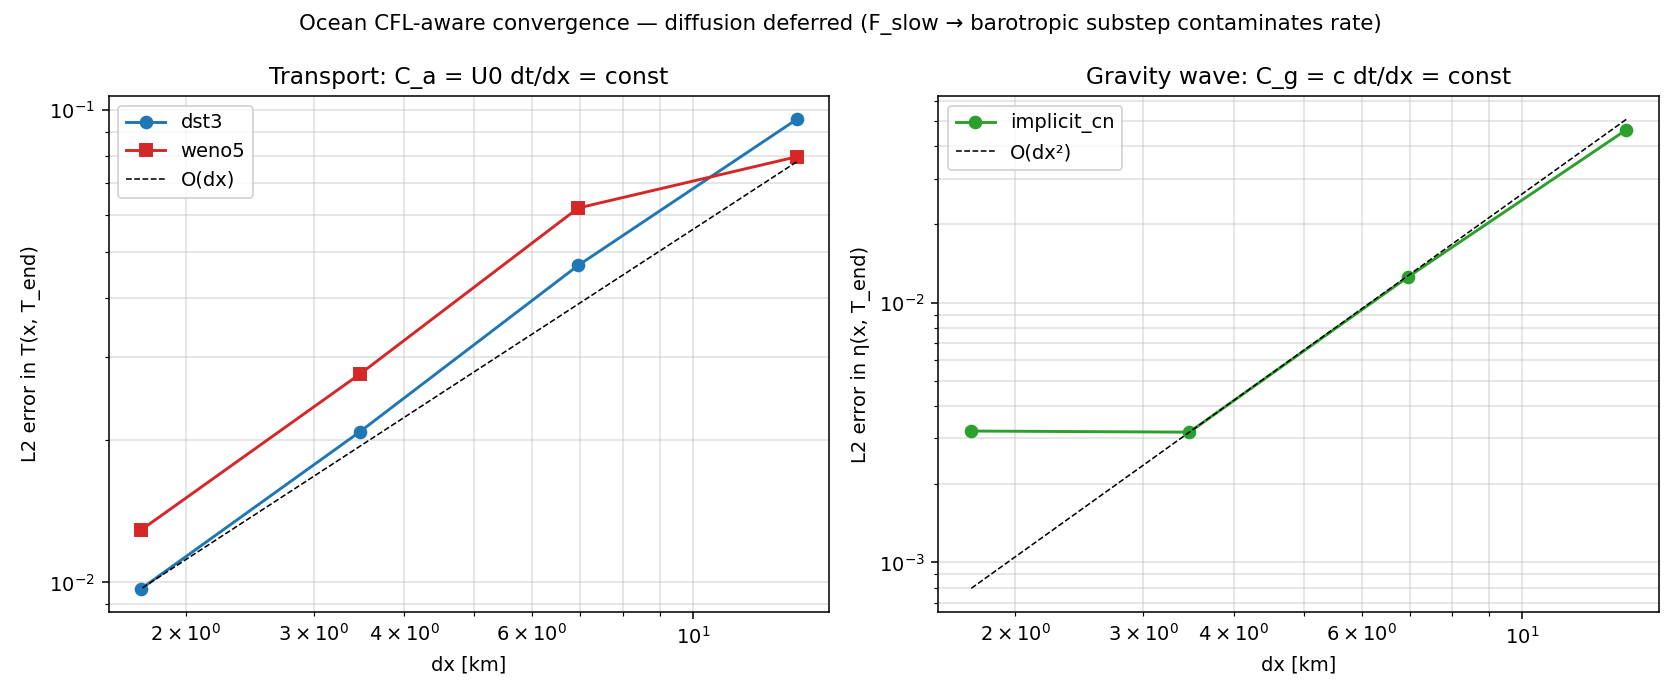
\includegraphics[width=\textwidth]{si_cfl_ocean.png}\caption{Ocean}\end{subfigure}
\caption{CFL-aware convergence: gravity-wave and transport errors vs.\ grid spacing with design-order
reference slopes.}\label{si:cfl}
\end{figure}

% =====================================================================
\clearpage
\bibliographystyle{unsrtnat}
\bibliography{references}

\end{document}
